\documentclass{article}
\usepackage{amsmath}
\usepackage{amsfonts, amsthm, amssymb}
\usepackage{graphicx}
\usepackage[colorlinks]{hyperref}
\usepackage[parfill]{parskip}
\usepackage{algorithm}
\usepackage{algorithmic}
\usepackage{enumerate}
\usepackage[shortlabels]{enumitem}
\usepackage{fullpage}
\usepackage{mathtools}

\usepackage{natbib}
\renewcommand{\bibname}{REFERENCES}
\renewcommand{\bibsection}{\subsubsection*{\bibname}}

\DeclarePairedDelimiterX{\norm}[1]{\lVert}{\rVert}{#1}

\newcommand{\eqdist}{\ensuremath{\stackrel{d}{=}}}
\newcommand{\Graph}{\mathcal{G}}
\newcommand{\Reals}{\mathbb{R}}
\newcommand{\Identity}{\mathbb{I}}
\newcommand{\distiid}{\overset{\text{i.i.d}}{\sim}}
\newcommand{\convprob}{\overset{p}{\to}}
\newcommand{\convdist}{\overset{w}{\to}}
\newcommand{\Expect}[1]{\mathbb{E}\left[ #1 \right]}
\newcommand{\Risk}[2][P]{\mathcal{R}_{#1}\left[ #2 \right]}
\newcommand{\Prob}[1]{\mathbb{P}\left( #1 \right)}
\newcommand{\iset}{\mathbf{i}}
\newcommand{\jset}{\mathbf{j}}
\newcommand{\myexp}[1]{\exp \{ #1 \}}
\newcommand{\abs}[1]{\left \lvert #1 \right \rvert}
\newcommand{\restr}[2]{\ensuremath{\left.#1\right|_{#2}}}
\newcommand{\ext}[1]{\widetilde{#1}}
\newcommand{\set}[1]{\left\{#1\right\}}
\newcommand{\seq}[1]{\set{#1}_{n \in \N}}
\newcommand{\dotp}[2]{\langle #1, #2 \rangle}
\newcommand{\floor}[1]{\left\lfloor #1 \right\rfloor}
\newcommand{\Var}{\mathrm{Var}}
\newcommand{\Cov}{\mathrm{Cov}}
\newcommand{\diam}{\mathrm{diam}}

\newcommand{\emC}{C_n}
\newcommand{\emCpr}{C'_n}
\newcommand{\emCthick}{C^{\sigma}_n}
\newcommand{\emCprthick}{C'^{\sigma}_n}
\newcommand{\emS}{S^{\sigma}_n}
\newcommand{\estC}{\widehat{C}_n}
\newcommand{\hC}{\hat{C^{\sigma}_n}}
\newcommand{\vol}{\mathrm{vol}}
\newcommand{\spansp}{\mathrm{span}~}
\newcommand{\1}{\mathbf{1}}

\newcommand{\Linv}{L^{\dagger}}
\DeclareMathOperator*{\argmin}{argmin}
\DeclareMathOperator*{\argmax}{argmax}

\newcommand{\emF}{\mathbb{F}_n}
\newcommand{\emG}{\mathbb{G}_n}
\newcommand{\emP}{\mathbb{P}_n}
\newcommand{\F}{\mathcal{F}}
\newcommand{\D}{\mathcal{D}}
\newcommand{\R}{\mathcal{R}}
\newcommand{\Rd}{\Reals^d}

%%% Vectors
\newcommand{\thetast}{\theta^{\star}}

%%% Matrices
\newcommand{\X}{X} % no bold
\newcommand{\Y}{Y} % no bold
\newcommand{\Z}{Z} % no bold
\newcommand{\Lgrid}{L_{\grid}}
\newcommand{\Dgrid}{D_{\grid}}
\newcommand{\Linvgrid}{L_{\grid}^{\dagger}}

%%% Sets and classes
\newcommand{\Cset}{\mathcal{C}}
\newcommand{\Csig}{\Cset_{\sigma}}
\newcommand{\Xset}{\mathcal{X}}
\newcommand{\Sset}{\mathcal{S}}
\newcommand{\Hclass}{\mathcal{H}}
\newcommand{\Pclass}{\mathcal{P}}
\newcommand{\domain}{\mathcal{X}}

%%% Distributions and related quantities
\newcommand{\Pbb}{\mathbb{P}}
\newcommand{\Ebb}{\mathbb{E}}
\newcommand{\Qbb}{\mathbb{Q}}
\newcommand{\Cbb}{\mathbb{C}}

%%% Functionals
\newcommand{\cut}{\textrm{cut}}

%%% Operators
\newcommand{\Tadj}{T^{\star}}
\newcommand{\dive}{\mathrm{div}}
\newcommand{\dif}{\mathop{}\!\mathrm{d}}
\newcommand{\Partial}{\mathcal{D}}
\newcommand{\Hessian}{\mathcal{D}^2}

%%% Misc
\newcommand{\grid}{\mathrm{grid}}
\newcommand{\critr}{R_n}
\newcommand{\dx}{\,dx}
\newcommand{\dy}{\,dy}
\newcommand{\dr}{\,dr}
\newcommand{\dxpr}{\,dx'}
\newcommand{\dypr}{\,dy'}
\newcommand{\wt}[1]{\widetilde{#1}}
\newcommand{\dist}{\mathrm{dist}}

%%% Order of magnitude
\newcommand{\soom}{\sim}

% \newcommand{\span}{\textrm{span}}

\newtheoremstyle{alden}
{6pt} % Space above
{6pt} % Space below
{} % Body font
{} % Indent amount
{\bfseries} % Theorem head font
{.} % Punctuation after theorem head
{.5em} % Space after theorem head
{} % Theorem head spec (can be left empty, meaning `normal')

\theoremstyle{alden} 


\newtheoremstyle{aldenthm}
{6pt} % Space above
{6pt} % Space below
{\itshape} % Body font
{} % Indent amount
{\bfseries} % Theorem head font
{.} % Punctuation after theorem head
{.5em} % Space after theorem head
{} % Theorem head spec (can be left empty, meaning `normal')

\theoremstyle{aldenthm}
\newtheorem{theorem}{Theorem}
\newtheorem{conjecture}{Conjecture}
\newtheorem{lemma}{Lemma}
\newtheorem{example}{Example}
\newtheorem{corollary}{Corollary}
\newtheorem{proposition}{Proposition}
\newtheorem{assumption}{Assumption}
\newtheorem{remark}{Remark}


\theoremstyle{definition}
\newtheorem{definition}{Definition}[section]

\theoremstyle{remark}

\begin{document}
\title{Thesis Proposal}
\author{Alden Green}
\date{\today}
\maketitle

\begin{abstract}
	In the classical data analysis setting, where we observe i.i.d. point-cloud data sampled from an unknown distribution $\Pbb$, there has been recent interest in the design and analysis of procedures which involve the geometry of $\Pbb$. Broadly speaking, these procedures either estimate geometric properties such as high-density regions of $\Pbb$, or leverage the geometry of $\Pbb$ in some downstream statistical learning task. One way to implicitly adapt to the geometry of $\Pbb$ is through the use of graph-based spectral methods. The underlying intuition is that when one appropriately constructs a neighborhood graph, the resulting graph Laplacian encodes a great deal of information about the geometry of $\Pbb$; for example, one can view its top eigenvectors as (discrete versions of) functions which are smooth with respect to $\Pbb$. For this reason, there has been extensive analysis on consistency properties of graph Laplacians, that is, in what ways and with what error they approximate continuum-level operators.
	
	\vspace{.02 in}
	
	In this thesis we will take a different approach, and analyze the effectiveness with which spectral algorithms perform traditional statistical learning tasks such as density clustering and hypothesis testing. In the density clustering problem, we consider a local version of spectral clustering using the Personalized PageRank (PPR) algorithm. We show that when a density cluster satisfies a natural set of geometric conditions PPR will provably recover it with high probability; we also derive lower bounds conversely showing that PPR will fail to recover geometrically poorly conditioned density clusters. In the hypothesis testing context, in some preliminary work we define a goodness-of-fit test using spectral-based test statistics formed over a neighborhood graph, and prove that it achieves minimax optimal testing rates against a certain class of smooth alternatives. We propose various extensions of this test targeted for wider classes of alternatives, and for the two-sample problem.
\end{abstract}


\section{Introduction and background.}

This document details the work I intend to complete for my thesis, and is separated into three sections. In the first section, I give background on the convergence properties of neighborhood graphs, as well as the statistical learning problems of clustering and hypothesis testing. In the second section, I detail work I have already completed on clustering using the local spectral algorithm PPR over neighborhood graphs. In the third section, I propose several statistics used to test hypotheses using the spectra of neighborhood graphs, and make explicit the ways in which I will investigate and characterize their behavior. Finally, I give an estimated timeline for completing my proposed work.

\subsection{Neighborhood graphs and their spectra.}
\label{subsec:neighborhood_graphs_spectra}

Let $X = \{x_1,
\ldots, x_n\}$ be a sample drawn i.i.d. from a distribution $\Pbb$ on $\Rd$,
with density~$f$.  For a radius $r > 0$, we define $G_{n,r}=(V,E)$ to be the
\emph{$r$-neighborhood graph} of $X$, an unweighted, undirected graph with
vertices $V=X$, and an edge $(x_i,x_j) \in E$ if and only if $\norm{x_i -
	x_j} \leq r$, where $\norm{\cdot}$ is the Euclidean norm. We denote by $A \in
\Reals^{n \times n}$ the adjacency matrix, with entries $A_{uv} = 1$ if
$(u,v) \in E$ and $0$ otherwise.  We also denote by $D$ the diagonal degree
matrix, with entries $D_{uu} := \sum_{v \in V} A_{uv}$, and by $I$ the $n
\times n$ identity matrix.

Spectral graph theory involves the study of the eigenvalues and eigenvectors of the graph Laplacian $L := D - A$\footnote{Also the normalized Laplacian matrices $L_{\textrm{rw}} = I - D^{-1}A$ and $L_{\textrm{n}} = D^{1/2}L_{\textrm{rw}}D^{-1/2}$.} and is broadly applicable to fields as diverse as the theory of randomized algorithms and differential geometry \citet{chung97}. 

When specifically considering Laplacians of neighborhood graphs such as $G_{n,r}$, one well-developed line of work concerns the asymptotic convergence properties of the various graph Laplacians to associated continuum Laplace operators. Let $\mathcal{X} \subseteq \Reals^d$ be an open, bounded, and connected set with Lipschitz boundary. The Laplace operator $\Delta: C^2(\mathcal{X}) \to L^2(\mathcal{X})$ is defined as
\begin{equation*}
\Delta g = - \dive(\nabla g) =: \sum_{i = 1}^{d} \frac{\partial^2 g}{\partial x_i^2}.
\end{equation*}
There are several ways in which the matrix $L$ can be said to be converging to the operator $\Delta$. The first of these is \emph{functional} convergence. Here, we think of $L$ as acting on functions in $\Reals^d$,
\begin{equation*}
Lg(x) := \frac{1}{n^2r_n^{d+2}}\sum_{i = 1}^{n}(g(x) - g(x_i))A_{ij}
\end{equation*}
and ask whether $Lg(x) \to \Delta g(x)$ in probability as $n \to \infty$ and $r_n \to 0$.  \citet{belkin03,belkin05} consider a slightly different neighborhood graph than $G_{n,r}$ (constructed with a Gaussian rather than uniform kernel) and show that when $\Pbb$ is the uniform distribution over $\mathcal{X}$, such a functional convergence occurs. \footnote{For this and many of the results summarized in this section, $\mathcal{X}$ is permitted to be a low-dimensional manifold, and $\Delta$ is then taken to be the Laplace-Beltrami operator.} \citet{singer06,gine06} extend these results by proving faster convergence rates and a uniform CLT, respectively. When $\Pbb$ is non-uniform the story is slightly different. Now the relevant continuum operator is a weighted analogue of the Laplace operator,
\begin{equation*}
\Delta_{\Pbb} g := - \frac{1}{f} \dive(f^2 \nabla g);
\end{equation*}
\citet{lafon04,hein05} prove the functional convergence $Lg(x) \to \Delta_{\Pbb} g(x)$ in probability as $n \to \infty$ as $n \to \infty$ and $r_n \to 0$.

Another mode of convergence is \emph{smoothness functional} convergence. In this case, we denote $\theta = (g(x_1),\ldots,g(x_n)) \in \Reals^n$, consider the smoothness functional
\begin{equation*}
S(g;\Pbb) := \int_{\mathcal{X}} \norm{\nabla g}_2^2~ f^2(x) \,dx
\end{equation*}
and ask whether $\frac{1}{n^2r_n^{d+2}}\theta^T L \theta \to S(g;\Pbb)$ in probability as $n \to \infty$ and $r_n \to 0$. \citet{bousquet03} proves that the smoothness functional converges pointwise--meaning for a fixed $g \in C^2(\mathcal{X})$--and \citet{hein06} extends this to show uniform convergence over a suitably chosen Holder ball.

The final mode of convergence we mention is \emph{spectral} convergence.  $\Delta_{\Pbb}$ is a positive semidefinite self-adjoint operator, and therefore has a discrete spectrum. Label the $i$th smallest eigenvalue of $\Delta_{\Pbb}$ as $\lambda_i$, with associated eigenfunction $u_i$; similarly, label the $i$th smallest eigenvalue of $L$ as $s_i$ with associated eigenvector $v_i$. We say $L$ converges spectrally to $\Delta_{\Pbb}$ if for any fixed $k \in \mathbb{N}$,
\begin{equation*}
\lim_{n \to \infty} s_{k} = \lambda_k, \quad \textrm{and} \quad \lim_{n \to \infty} \frac{1}{n}\sum_{i = 1}^{n} (u_k(x_i) - v_{k,i})^2 = 0
\end{equation*}
where the limits are taken in probability. \citet{vonluxburg2008} consider the case of a fixed $r_n = r$, and prove spectral convergence of $L$ to an appropriately defined integral operator, \citet{belkin07} prove that when $\Pbb$ is the uniform distribution over $\mathcal{X}$, $L$ converges spectrally to $\Delta_{\Pbb} = \Delta$ for some $r_n \to 0$ as $n \to \infty$, and \citet{garciatrillos18} extend this result to hold for general $\Pbb$ and obtain rates at which $r_n$ may converge to $0$. 

The convergence of graph Laplacians to underlying continuum differential operators suggests they may be used to perform a variety of desirable tasks in statistical learning. In this thesis proposal, we study a few of these tasks in detail, and show how spectral methods can be used to perform the statistical tasks of density clustering and nonparametric hypothesis testing. Before doing so, we provide some background on each of these areas.
	 
%\begin{itemize}
	%\item Dimension reduction: under the hypothesis that the data lie on, or are concentrated near, a manifold $\mathcal{M} \subset \Reals^d$ of dimension $m < d$, the eigenvectors $v_1,\ldots,v_m$, can be used to embed $x_i \mapsto (v_{i,1},\ldots v_{i,m})$, reducing the dimension from $d$ to $m$ without losing the geometric structure of $\Pbb$. This algorithm is known as Laplacian Eigenmaps \citet{belkin03a}. 
	%\item Clustering: under the hypothesis that the distribution $\Pbb$ is approximately supported on disjoint connected components $\mathcal{C}_1,\ldots,\mathcal{C}_k$, the embedding $x_i \mapsto (v_{i,1},\ldots,v_{i,k})$ will reveal the cluster structure of $\Pbb$. Subsequent application of a simple clustering method such as $k$-means clustering will then correctly partition the data $X$ into clusters \cite{ng01,ariascastro11,shi2009}.
	%\item Semi-supervised and supervised learning: Discuss the study of Laplacians in supervised learning \textcolor{red}{(Bousquet + Chapelle, Lee + Izbicki, GarciaTrillos + Murray, Padilla)} Discuss the study of Laplacians in semi-supervised learning \textcolor{red}{(Belkin + Niyogi, Zhou + Belkin, Slepcev and Thorpe)}. 
%\end{itemize}

\subsection{Clustering.}

Clustering involves splitting a given data set
into groups that satisfy some notion of within-group similarity and
between-group difference. There are many ways to define different types of clusters; we review a few that are especially related to our work. 

\subsubsection{Density clustering.}

Let $X = \set{x_1,\ldots,x_n}$ consist of i.i.d. samples drawn from a distribution $\Pbb$ on $\Reals^d$, with density $f$. The \emph{density clusters} of $f$, defined as the connected components of
the upper level set $\{x \in \Rd : f(x) \geq \lambda\}$ for some $\lambda > 0$
are a central object of interest in the statistical clustering literature, dating
back to the work of \citet{hartigan1981}, who shows that the classical single-linkage hierarchical clustering algorithm is guaranteed to recover density clusters only when $d = 1$. \citet{polonik1995, rigollet2009} study density clustering under the 
symmetric set difference metric, \citet{tsybakov1997, singh2009} describe
minimax optimal level-set estimators under Hausdorff loss and
\citet{hartigan1981, chaudhuri2010, balakrishnan2013,kpotufe11} consider consistent estimation of the
cluster tree. None of these works, however, study the ability of spectral algorithms to recover density clusters, which will be our focus in Section~\ref{sec:density_clustering_PPR}.

\subsubsection{Nonparametric mixture model.}

The results in Section~\ref{subsec:neighborhood_graphs_spectra} have straightforward consequences for the consistency of spectral clustering (for instance, see \cite{vonluxburg2008,garciatrillos18}). However, the behavior of the spectra of these continuum operators can in general be hard to grasp. Therefore, further work relating this spectra to the geometry of the distribution $\Pbb$ is of interest. In this spirit, \citet{shi2009,schiebinger2015,garciatrillos19,ariascastro11} examine the ability of spectral algorithms to recover the latent labels in certain geometrically well-conditioned nonparametric mixture models $\Pbb = \sum_{i = 1}^{k} \pi_i \Pbb_i$. These results focus on global rather than local 
methods, and thus impose global rather than local conditions on the nature
of the density. Moreover, they do not in general guarantee recovery of density 
clusters, which is the focus in our work. Perhaps most importantly, these works
rely on general cluster saliency conditions, which implicitly depend on many
distinct geometric aspects of the cluster $\Cset$ under consideration. We will make
this dependence more explicit, and in doing so expose the role each geometric
condition plays in the clustering problem. 

\subsubsection{Worst-case analysis.}
\label{subsubsec:worst_case_analysis}

An altogether different approach is to treat the graph $G = (V,E)$ as fixed, rather than as a random geometric graph formed over data as is the case when $G = G_{n,r}$. Now, the quality of the clustering algorithm necessarily depends on the extent to which $G$ contains natural clusters. To quantify the \textcolor{red}{clusterability} of a given subset $S \subseteq V$, let the normalized cut $\Phi(S;G)$ be given by
\begin{equation*}
\Phi(S;G) = \frac{\cut(S;G)}{\min\{\vol(S;G), \vol(S^c;G)\}},\quad \cut(S;G) := \sum_{u \in S} \sum_{w \in S^c} A_{uv}, \quad \vol(S;G) = \sum_{u \in S} D_{uu}.
\end{equation*}
and the conductance $\Psi(S;G)$ be 
\begin{equation*}
\Psi(S;G) = \min_{A \subset S} \Phi(A;G[S])
\end{equation*}
where $G[S] = (S,E_S), E_S = E \cap (S \times S)$ is the subgraph of $G$ induced by $S$. The normalized cut and conductance functionals measure the external connectivity of $S$ to the rest of $G$, and the internal connectivity of $G[S]$, respectively. \cite{kannan04} assume there exists a partition $S_1 \cup \ldots \cup S_k$ such that $\Phi(S_j) \leq \phi$ and $\Psi(S_j) \geq \psi$ for all $j$. They analyze an algorithm which recursively splits the graph $G$ based on its eigenvectors, resulting in clusters $C_1 \cup \ldots \cup C_k = V$, and prove upper bounds on the normalized cuts $\Phi(C_j)$ and conductances $\Psi(C_j)$ in terms of $\phi$ and $\psi$. \citet{spielman2013,andersen2006} consider the local clustering problem, where assumptions are made only with respect to some small subset $S \subseteq V$. They each consider random walk based algorithms which cluster using locally-biased spectra, and derive upper bounds on the normalized cut of the outputted cluster $\Phi(C)$ in terms of $\Phi(S)$. \cite{zhu2013} extends this analysis, showing that improvements in the quality of a cluster estimate are possible when $\Psi(S) > \Phi(S)$. We rely on the analysis of \cite{zhu2013} in our work; however, our setting is quite different, as we work with respect to the random graph $G_{n,r}$ rather than a fixed $G$, and seek to derive bounds which depend on the distribution $\Pbb$ rather than on $\Phi$ and $\Psi$, which in our context are random functionals.

\subsection{Nonparametric hypothesis testing.}

In hypothesis testing, the goal is distinguish whether our data are generated from some null model -- generally a simple model displaying a lack of meaningful structure -- or an alternative model. \emph{Regression} and \emph{density} testing are two related but distinct hypothesis testing problems. We will formally introduce each problem and provide some relevant background. Additionally, we will cover some common classes of test statistics used for nonparametric hypothesis testing.

\subsubsection{Regression testing.}

In addition to observing i.i.d samples $x_1,\ldots,x_n$ from a distribution $\mathbb{P}$ with density $p$ supported on $\mathcal{X} := [0,1]^d \subset \Reals^d$\footnote{For the purposes of this proposal, whenever we discuss hypothesis testing we will assume $\mathcal{X} = [0,1]^d$, i.e. the unit cube with dimension equal to that of the ambient space $\Reals^d$.}, suppose we observe $Y = \set{y_1,\ldots,y_n}$ according to the following regression model:
\begin{equation}
\label{eqn:regression}
y_i = f(x_i) + \varepsilon_i, \quad \varepsilon_i \overset{\textrm{i.i.d}}{\sim} \mathcal{N}(0,1)
\end{equation}
We wish to distinguish
\begin{equation*}
\mathbf{H}_0: f = f_0 := 0 \quad \textrm{vs} \quad \mathbf{H}_{\textrm{a}}: f \neq f_0
\end{equation*}
We will evaluate our performance using worst-case risk: for a given function class $\mathcal{H}$ and test function $\phi: \Reals^n \to \set{0,1}$, let
\begin{equation*}
\mathcal{R}(\phi; \mathcal{H}) = \Ebb_{f = f_0}(\phi) + \sup_{f \in \mathcal{H}, f \neq f_0} \Ebb_f(1 - \phi).
\end{equation*}
Without further assumptions on $\mathcal{H}$ no test achieves meaningful power uniformly over all $f \in \mathcal{H}$ \citet{janssen2000}; to make the hypothesis testing question well-posed we will therefore restrict the function class $\mathcal{H}$ in two standard ways. One, when considering type II error we will remove a radius-$\epsilon$ ball in the $L_2$ norm around $f_0$ and consider only the remaining functions
\begin{equation*}
\mathcal{H}_{\epsilon} := \set{f \in \mathcal{H}:\norm{f - f_0}_2 > \epsilon}.
\end{equation*}
Otherwise we can always pick a function $f \neq f_0$ in $\mathcal{H}$ which is indistinguishable from $f_0$ given a finite number of samples. Two, we will insist that the functions in $\mathcal{H}$ display some degree of regularity or smoothness; otherwise it may not be possible to consistently estimate the functional $\norm{f - f_0}_2$. 

Let $\alpha \in (0,1)$ be a user input specifying a tolerated level of testing error. A typical way to characterize the performance of a test $\phi$ is through the critical radius $\epsilon_n(\phi; \mathcal{H})$, defined as
\begin{equation*}
\epsilon_n(\phi; \mathcal{H}) = \inf\{\epsilon: \mathcal{R}(\phi; \mathcal{H}_{\epsilon}) \leq \alpha\}.
\end{equation*}
We can then measure the difficulty of a given problem through the minimax critical radius $\epsilon_n^{\star}$, formally 
\begin{equation*}
\epsilon_n^{\star}(\mathcal{H}) = \inf \set{\epsilon:\inf_{\phi} \mathcal{R}(\phi; \mathcal{H}_{\epsilon} ) \leq \alpha},
\end{equation*}
where the infimum is over all Borel measurable functions $\phi: \Reals^n \to \set{0,1}$. We say a test $\phi$ is minimax optimal over a function class $\mathcal{H}$ if $\epsilon_n(\phi; \mathcal{H}) \asymp \epsilon_n^{\star}(\mathcal{H})$, and we call the rate at which $\epsilon_n^{\star}(\mathcal{H}) \to 0$ as a function of $n$ the \emph{minimax testing rate} over $\mathcal{H}$. To concisely state rates, we will use order notation, in which we write $a_n = O(b_n)$ when $a_n \leq c b_n$ for some constant $c$ and all $n \in \mathbb{N}$, $a_n = o(b_n)$ when $a_n/b_n \to 0$ as $n \to \infty$, and $a_n \asymp b_n$ when $c b_n \leq a_n \leq C b_n$ for constants $c$ and $C$ and all $n \in \mathbb{N}$.

\paragraph{Testing over Sobolev spaces.}
The first type of function class $\mathcal{H}$ we consider will be balls in Sobolev spaces. We say a Borel measurable function $f: \mathcal{X} \to \Reals$ is in the space $\mathcal{L}^p(\mathcal{X})$ for $1 \leq p < \infty$ if 
$\norm{f}_{\mathcal{L}^p(\mathcal{X})} := \int_{\mathcal{X}} \abs{f(x)}^p \,dx < \infty$. Then, the Sobolev space $W_d^{s,2}(\mathcal{X})$ consists of all functions $f \in \mathcal{L}^2(\mathcal{X})$ such that for each $\alpha = (\alpha_1,\ldots,\alpha_d)$ with $\abs{\alpha} := \sum_{i = 1}^{d} \alpha_i \leq s$, the weak derivative $D^{\alpha}f$ (See \citet{evans10} for a formal definition) belongs to $\mathcal{L}^2(\mathcal{X})$. The Sobolev $\{s,2\}$ norm is then 
\begin{equation*}
\norm{f}_{W_d^{s,2}(\mathcal{X})}^2 = \sum_{\abs{\alpha} \leq s} \int_{\mathcal{X}} \abs{D^{\alpha}f}^2 \,dx
\end{equation*}
and for a given $L > 0$, the corresponding ball is $W_d^{s,2}(\Xset; L) = \set{f: \norm{f}_{W^{s,2}(\Xset)} \leq L}$. (In this work, we will treat $L$ as a fixed, known constant.)

Minimax testing rates for the Sobolev regression testing problem in one dimension were first derived by \citet{ingster82} for the idealized \emph{white noise} regression model:
\begin{equation}
\label{eqn:gaussian_white_noise}
\,dY(x) = f(x) \,dx + \frac{\sigma}{\sqrt{n}}\,dW(x)
\end{equation}
where $\,dW(x)$ denotes a Gaussian white noise process on $\mathcal{X} \subset \Reals$ (defined formally in \citet{gine16} Section 1.2) and $\sigma > 0$ is a known constant. In this case, the minimax test rate is $\epsilon_n^{\star}(\mathcal{W}_d^{s,2}(\mathcal{X}, L)) \asymp n^{-2s/(4s + 1)}$ for all values of $s > 0$. \citet{ingster05} extend this to the multivariate setting where $\mathcal{X} \subseteq \Reals^d$, and show that $\epsilon_n^{\star}(\mathcal{W}_d^{s,2}(\mathcal{X}, L)) \asymp n^{-2s/(4s + d)}$, again for all $d \geq 1, s > 0$. The case where we observe data according to the generative model~\eqref{eqn:regression} was treated in \cite{ingster09}, wherein it is shown that the minimax rate remains the same  $\epsilon_n^{\star}(\mathcal{W}_d^{s,2}(\mathcal{X}, L)) \asymp n^{-2s/(4s + d)}$ so long as $4s > d$. When $4s < d$, if we replace the assumption $f \in W_d^{s,2}(\mathcal{X},L)$ by the assumption $\left(\int_{\mathcal{X}} f^4(x) \,dx\right)^{1/4}$, then \citet{guerre02} show that a test $\phi$ based on the statistic $\frac{1}{n}\sum_{i = 1}^{n}y_i^2$ will have testing error on the order of $n^{-1/4}$ . Since $\mathcal{W}^{s,2}$ does not compactly embed into $\mathcal{L}^4$ when $4s < d$ this result does not apply to Sobolev spaces in this regime; indeed it seems likely that no uniformly consistent test exists over these spaces, as the function $f^2$ may no longer have finite variance.

\paragraph{Testing over Total Variation (TV) spaces.}

To one extent or another, functions in the Sobolev balls exhibit homogeneous smoothness. In reality we may not wish to restrict our attention to such functions. We therefore consider functions of bounded total variation. Formally, for a function $f \in L^1(\mathcal{X})$ the \emph{total variation} semi-norm of $f$ is \citet{evans15}
\begin{equation*}
TV(f;\mathcal{X}) := \sup \left\{ \int_{\mathcal{X}} f \, \dive \, \psi \,dx : \psi \in C_c^1(\mathcal{X}; \Reals^d), \abs{\psi} \leq 1 \right\};
\end{equation*}
and we write $BV_d(\mathcal{X})$ for the subset of functions $f \in L^1(\mathcal{X})$ which have bounded norm
\begin{equation*}
\norm{f}_{BV_d(\mathcal{X})} := \norm{f}_{\infty} + TV(f;\mathcal{X}).
\end{equation*}

In the one-dimensional case, some work has been done on nonparametric testing over the Besov spaces $B_{p,q}^s(\mathcal{X})$ (for a formal definition see Section 4.3 of \cite{gine16}), which we can relate to the bounded variation space $BV_1(\mathcal{X})$ via the embeddings
\begin{equation}
\label{eqn:besov_embeddings}
B_{11}^1(\mathcal{X}) \subseteq BV_1(\mathcal{X}) \subseteq B_{1\infty}^1(\mathcal{X}).
\end{equation}

\citet{lepski1999} study the regression testing problem, with data observed according to the white noise model as in \eqref{eqn:gaussian_white_noise}. They derive among other things that for the Besov balls $B_{1,q}^s(\mathcal{X}; L)$, the minimax critical radius $\epsilon_n^{\star}(B_{1,q}^s(\mathcal{X}; L)) \asymp n^{-2s'/(4s' + 1)}$, where $s' = s - \frac{1}{4}$ and the result holds for any $s > 1, q \geq 1$. \citet{ingster00} improve on this by showing the same result holds whenever $s > 1/2$. This along with~\eqref{eqn:besov_embeddings} implies that $\epsilon_n^{\star}(BV_1(\mathcal{X})) \asymp n^{-\frac{3}{8}}$. 

When $d \geq 2$ minimax testing rates over the Besov and bounded variation spaces are still unknown. However, study of the equivalent estimation problem suggests the answers may be substantially different from the 1d problem. \citet{sadhanala16} consider a discretized version of this problem -- where observations are made on a discrete grid and the regression function is assumed to lie within a discrete bounded variation class -- and show that the minimax estimation rate in empirical norm is on the order of $n^{-1/d}$ for $d \geq 2$. This is slower than minimax estimation rate over the Sobolev space $\mathcal{W}_d^{1,2}$, the largest Sobolev space inscribed within $BV_d$. \citet{delyon96,kerkyacharian08,lepski2015,ruiz18} all consider the regression white noise model \eqref{eqn:gaussian_white_noise} and show, in progressive degrees of generality, that the minimax rates over the Besov spaces $B_{p,q}^s$ exhibit a phase transition at the boundary $2s = d$. When $2s > d$, the minimax estimation rate (with loss measured in $\mathcal{L}^2$ norm) is the standard $n^{-s/(2s + d)}$; on the other hand when $2s < d$, the minimax rate is $n^{-s/2d}$ which is much slower. When $s = 1$, this phase transition occurs at $d = 2$, and so in a minimax sense the univariate and multivariate estimation problems over $BV_d$ are revealed to be quite different. \citet{sadhanala17} show that this same phenomenon carries over to the grid, and the discrete TV classes defined upon it. 


\subsubsection{Density testing.}
\label{subsubsec:density_testing}

In the two-sample density testing problem, we observe independent samples $Z = z_1,\ldots,z_N \sim \Pbb$ and $Y = y_1,\ldots,y_M \sim \Qbb$, where $\Pbb$ and $\Qbb$ are distributions over $\Reals^d$ with densities $p$ and $q$, respectively. Our goal is to distinguish the hypotheses
\begin{equation*}
\mathbf{H}_0: \Pbb = \Qbb \quad \textrm{vs} \quad \mathbf{H}_{\textrm{a}}: \Pbb \neq \Qbb
\end{equation*}
and we again evaluate our performance using worst-case risk; letting $\phi:\Reals^{N + M} \to \{0,1\}$, 
\begin{equation*}
\mathcal{R}(\phi; \mathcal{H}) = \inf_{p \in \mathcal{H}}\Ebb_{p,p}(\phi) + \sup_{p \neq q, p,q \in \mathcal{H}} \Ebb_{p,q}(1 - \phi),
\end{equation*}
and the critical radius $\epsilon_n$. (Although we overload notation by having $\mathcal{R}$ and $\epsilon_n$ refer to the worst-case risk and critical radius in both the regression and density testing problems, it will always be clear from context which problem we are referring to.)

\paragraph{Testing over Holder spaces.} Unlike in the regression testing context, where $f$ is assumed to belong to a Sobolev space, most of the study of density testing seems to have dealt with the case where $\mathcal{H}$ is a Holder space. For a given $s > 0$, the $s$th Holder norm is given by
\begin{equation*}
\norm{f}_{C_d^{s}(\mathcal{X})} := \sum_{\abs{\alpha} \leq s} \norm{D^{\alpha}f}_{\infty} + \sum_{\abs{\alpha} = s} \sup_{x,y \in \mathcal{X}} \frac{\abs{D^{\alpha}f(y) - D^{\alpha}f(x)}}{\norm{x - y}_2}
\end{equation*}
and the $s$th Holder space $C_d^{s}(\mathcal{X})$ consists of all functions which are $s$ times continuously differentiable with finite $s$ Holder norm. Denote the Holder unit ball by $C_d^{s}(\mathcal{X},L) = \set{f \in C_d^{s}(\mathcal{X}): \norm{f}_{C_d^{s}(\mathcal{X})} \leq L}$.

\citet{ingster87} considers the 1d version of the problem and shows that the minimax critical radius for the Holder balls $C_d^{s}(\mathcal{X};L)$ is $\epsilon_n^{\star}(C^{s}(\mathcal{X};L)) \asymp n^{-2s/(4s + 1)}$. This means that the Holder space $C_d^{s}(\mathcal{X})$ and the smallest Sobolev space it compactly embeds into, $W_d^{s,2}(\mathcal{X})$, have the same minimax testing rates in the density and regression testing problems, respectively. \cite{ariascastro18} examines the multivariate version of the problem and derives the rate $\epsilon_n^{\star}(C_d^{s}(\mathcal{X};L)) \asymp n^{-2s/(4s + d)}$. In both cases, the stated rates hold for all $s > 0$, and in the second case for all $d \geq 1$. 

Using asymptotic equivalence results \citet{reiss08,nussbaum96,brown96} between the density and regression setups, and sampling and Gaussian white noise models, we can infer some results about minimax rates over Sobolev classes in the former from those in the latter. However, to the best of our knowledge, the density testing problem over Sobolev spaces has not been directly studied.

\subsubsection{Background on nonparametric test statistics.}

The $\chi^2$-test is a classical two-sample test, in which the domain $\mathcal{X}$ is partitioned into bins $B_1,\ldots,B_\kappa$ where $\kappa \in \mathbb{N}$ is a tuning parameter. Letting $\mathbb{P}_N$ be the empirical distribution of $Z$, and likewise for $\mathbb{Q}_M$ and $Y$, the resulting statistic can be expressed as 
\begin{equation}
\label{eqn:chi_squared}
T_{\chi^2} := \sum_{k = 1}^{\kappa} \left(\frac{\mathbb{P}_N(B_k) - \mathbb{Q}_M(B_k)}{\mathbb{P}_N(B_k) + \mathbb{Q}_M(B_k)}\right)^2.
\end{equation}
The upper bounds in the density testing problem discussed in the previous section are derived using an unnormalized version of $T_{\chi^2}$. In addition to the $\chi^2$-test, there are several classes of test statistics used to perform nonparametric hypothesis testing which are worthy of our attention.

\paragraph{Edge-counting.}
In the two-sample density testing problem, \citet{schilling86, bhattacharya15} analyze edge-counting statistics, where a $k$NN graph $G_{n,k}$ is formed over all the samples $X = (z_1,\ldots,z_N,y_1,\ldots,y_M)$ (where $n = M + N$ is the total number of samples) and the statistic considered is then
\begin{equation}
\label{eqn:edge_count_statistic}
T_{\textrm{edge}} := \sum_{i = 1}^{N} \sum_{j = 1}^{M} \1(z_i \sim y_j \textrm{ in } G_{n,k}).
\end{equation}
While there are some similarities between $T_{\mathrm{edge}}$ and the statistic $T_{\mathrm{spec}}$ we propose and analyze later in Section~\ref{subsec:spectral_regression_testing}, they are quite distinct. For one, they depend on different constructions of the neighborhood graph; perhaps more fundamentally, they use the spectrum of the resulting neighborhood graphs in different ways. Preliminary results (see Figure~\ref{fig:fig3}) show that these differences in construction lead to empirically different behavior over a range of testing problems.

\paragraph{Truncated-series.}

In the regression testing problem, \citet{ingster09} upper bound the minimax testing rate by considering a truncated series test statistic, where the data is projected onto a subspace spanned by (evaluations of) low-frequency harmonics, and the test statistic is the empirical norm of this projection. Let $\set{\phi_j}$ be the standard Fourier basis in $L_2([0,1])$, meaning
\begin{equation*}
\phi_0(x) = 1,~~ \phi_j(x) = \sqrt{2}\cos(2\pi j u) ~~\textrm{for each $j \in \mathbb{Z}_{-}$},~~ \phi_j(x) = -\sqrt{2}\sin(2\pi j u) ~~\textrm{for each $j \in \mathbb{Z}_{+}$}:
\end{equation*}
The test statistic which \citet{ingster09} analyze is then
\begin{equation}
\label{eqn:harmonic}
T_{\mathrm{Harm}} := \frac{1}{n}\sum_{\ell,-\ell \in [\kappa]^d} \left(\sum_{i = 1}^{n} \phi_{\ell}(x_i) y_i\right)^2, \quad \textrm{where}~ \phi_{\ell}(x) = \prod_{i = 1}^{d} \phi_{\ell_i}(x_i)
\end{equation}
for $\ell \in \mathbb{Z}^d$, $x \in \Reals^d$, and 
$\kappa \in \mathbb{N}$ a tuning parameter. The test statistic $T_{\mathrm{spec}}$ which we propose and analyze in Section~\ref{subsec:spectral_regression_testing} is closely related to $T_{\mathrm{Harm}}$, the crucial difference being that instead of the Fourier basis $\set{\phi_{\ell}}$, which are eigenfunctions of the Laplacian operator $\Delta$, we use eigenvectors $\set{v_k}$ of the graph Laplacian matrix.

\paragraph{Integral Probability Metrics (IPMs).}

Much recent attention \citet{muller97,sriperumbudur09,gretton12,mroueh17} has been paid to IPMs, which are statistics of the form
\begin{equation*}
\sup_{f \in \mathcal{F}} \abs{\mathbb{P}_n f - \mathbb{Q}_n f}
\end{equation*}
used to perform two-sample density testing. (Here, $\mathcal{F}$ is appropriately chosen set of functions, for example $\mathcal{F}$ might be the unit ball in a Holder or Sobolev space). Of course, for any graph $G = (V,E)$, the corresponding incidence matrix $B$ induces a notion of smoothness for vectors $\theta \in \Reals^{\abs{V}}$. Formally for some $s,p \in \mathbb{N}$, let the smoothness functional $S_{s,p}(\theta) = \norm{B^{(s)}\theta}_p$ where
\begin{equation*}
B^{(s)} = 
\begin{cases}
L^{s/2}, & \textrm{when $s$ is even} \\
B L^{(s-1)/2}, & \textrm{when $s$ is odd.}
\end{cases}
\end{equation*}
Then the classes $\Theta_{s,p} := \set{\theta \in \Reals^n: S_{s,p}(\theta) \leq L}$ can be viewed as possessing various types of smoothness, analogous to function classes such as Sobolev or Holder classes. It is therefore natural to consider IPMs of the form
\begin{equation*}
\sup_{\theta \in \Theta_{s,p}} \abs{\mathbb{P}_N \theta - \mathbb{Q}_M \theta};
\end{equation*}
and we will propose a pair of such statistics in Section~\ref{sec:neighborhood_graph_IPMs}.

\section{Density clustering with PPR.}
\label{sec:density_clustering_PPR}

In our density clustering work, we examine the ability of Personalized PageRank (PPR) -- a local spectral algorithm-- to recover density clusters. First, we motivate and formally define the PPR clustering algorithm we subsequently analyze. 

\subsection{PPR clustering.}

When applied to geometric graphs built from a large number of samples,
global spectral clustering methods can be computationally cumbersome and   
insensitive to the local geometry of the underlying distribution
\citep{leskovec2010,mahoney2012}.  This has led to increased interest in
\emph{local} spectral clustering algorithms, which leverage locally-biased spectra
computed using random walks around some user-specified seed node.  A popular 
local clustering algorithm is the Personalized PageRank (PPR) algorithm, first introduced by 
\citet{haveliwala2003}, then further developed by
several others~\citep{spielman2011,spielman2014,andersen2006,mahoney2012,zhu2013}.

The PPR vector $p_v = p(v,\alpha;G_{n,r})$, based on
a seed node $v \in V$ and a teleportation parameter $\alpha \in [0,1]$, is defined to be 
the solution of the following linear system:
\begin{equation}
\label{eqn: ppr_vector}
p_v = \alpha e_{v} + (1 - \alpha) p W,
\end{equation}
where $W = \frac{1}{2}(I + D^{-1}A)$ is the lazy random walk matrix over
$G_{n,r}$ and $e_{v}$ is the indicator vector for node $v$ (that has a 1 in the
$v$-th position and 0 elsewhere).

\subsubsection{Sweep cut.}

We employ the sweep cut method to obtain a local cluster from the PPR embedding $p_v$. In more detail, for a level $\beta > 0$, we define a \emph{$\beta$-sweep cut} of $p_v = (p_v(u))_{u \in V}$
as   
\begin{equation}
\label{eqn: sweep_cuts}
S_{\beta,v} := \set{u \in V: \frac{p_v(u)}{D_{uu}} > \beta}.
\end{equation}
We will use the normalized cut metric to determine which sweep cut $S_{\beta}$
is the best cluster estimate. For a set $S \subseteq V$ with complement $S^c = V
\setminus S$, we define \smash{$\cut(S;G_{n,r}) := \sum_{u \in S, v \in S^c}
	A_{uv}$}, and \smash{$\vol(S; G_{n,r}) := \sum_{u \in S} D_{uu}$}.  We
define the \emph{normalized cut} of $S$ as
\begin{equation}
\label{eqn: normalized_cut}
\Phi(S; G_{n,r}) := \frac{\cut(S;G_{n,r})}{\min \set{\vol(S; G_{n,r}), \vol(S^c; G_{n,r})}}.
\end{equation}
Having computed sweep cuts $S_{\beta}$ over a range \smash{$\beta \in  
	(L, U)$} (where the range $(L,U)$ is also a user-specified parameter), we output the cluster estimate
\smash{$\widehat{C} = S_{\beta^*}$} that has minimum normalized cut.
%\smash{$\Phi(S_{\beta^*}; G_{n,r})$}. 
For concreteness, the PPR algorithm is summarized in Algorithm~\ref{alg: ppr}. 

\begin{algorithm}
	\caption{PPR on a neighborhood graph}
	\label{alg: ppr}	
	{\bfseries Input:} data $X=\{x_1,\ldots,x_n\}$, radius $r > 0$, teleportation
	parameter $\alpha \in [0,1]$, seed $v \in X$, sweep cut range $(L,U)$. \\     
	{\bfseries Output:} cluster $\widehat{C} \subseteq V$.
	\begin{algorithmic}[1]
		\STATE Form the neighborhood graph $G_{n,r}$.
		\STATE Compute the PPR vector $p_v=p(v, \alpha; G_{n,r})$ as in \eqref{eqn: 
			ppr_vector}. 
		\STATE For \smash{$\beta \in (L,U)$} compute sweep cuts 
		$S_{\beta}$ as in \eqref{eqn: sweep_cuts}.
		\STATE Return the cluster \smash{$\widehat{C} = S_{\beta^*}$}, where  
		$$
		\beta^* = \argmin_{\beta \in (L,U)}~ \Phi(S_{\beta}; G_{n,r}).
		$$
	\end{algorithmic}
\end{algorithm}

\subsection{Estimation of density clusters} 
Let \smash{$\Cbb_f(\lambda)$} denote 
the connected components of the density upper level set $\{x \in \Rd: f(x) >
\lambda\}$.  For a given density cluster \smash{$\Cset \in \Cbb_f(\lambda)$}, we
call $\Cset[X] = \Cset \cap X$ the \emph{empirical density cluster}. The size of the symmetric set difference between estimated and empirical cluster is 
a commonly used metric to quantify cluster estimation error
\citep{korostelev1993,polonik1995,rigollet2009}. We will consider a related metric, the volume of the symmetric set difference, which weights points according to their degree in $G_{n,r}$. 
\begin{definition}
	\label{def:volume_symmetric_set_difference}
	For an estimator $\widehat{C} \subseteq X$ and a set $\mathcal{S} \subseteq \Rd$, the symmetric set difference is 
	\begin{equation*}
	\widehat{C} \vartriangle \mathcal{S}[X] := \bigl(\widehat{C} \setminus \mathcal{S}[X]\bigr) \cup \bigl(\mathcal{S}[X]\setminus\widehat{C} \bigr).
	\end{equation*}
	We will measure the discrepancy between $\widehat{C}$ and $\mathcal{S}[X]$ by the volume of the symmetric set difference,
	\begin{equation*}
	\Delta(\widehat{C}, \mathcal{S}[X]) := \vol(\widehat{C} \vartriangle \mathcal{S}[X]; G_{n,r})
	\end{equation*}
\end{definition}
However, the symmetric set difference does not measure whether \smash{$\widehat{C}$} 
can distinguish any two distinct clusters \smash{$\Cset,\Cset' \in
	\Cbb_f(\lambda)$}. We therefore also study a second notion of cluster
estimation, first introduced by \citet{hartigan1981}, and defined
asymptotically. 

\begin{definition}[Consistent density cluster estimation]
	\label{def: consistent_density_cluster_estimation}
	For an estimator \smash{$\widehat{C} \subseteq X$} and cluster 
	\smash{$\Cset \in \Cbb_f(\lambda)$}, we say \smash{$\widehat{C}$} is a consistent 
	estimator of $\Cset$ if for all \smash{$\Cset' \in \Cbb_f(\lambda)$} with
	$\Cset \not= \Cset'$, the following holds as $n \to \infty$: 
	\begin{equation}
	\label{eqn: consistent_density_cluster_recovery}
	\Cset[X] \subseteq \widehat{C} \quad \text{and} \quad
	\widehat{C} \cap \Cset'[X] = \emptyset,
	\end{equation}
	with probability tending to 1.
\end{definition}
\noindent Consistent cluster recovery roughly ensures that, for a given density threshold $\lambda$, the estimated cluster $\widehat{C}$ contains all
points in a true
density cluster $\Cset \in \Cbb_f(\lambda)$, and simultaneously does not contain any points in any other density cluster $\Cset' \in \Cbb_f(\lambda)$. 

With these definitions in place, our broad goal will be to understand the extent to which the PPR algorithm is able to
recover a cluster which either guarantees low symmetric set difference to a true density cluster, or which consistently estimates
a true density cluster.

\subsection{Geometric Conditioning of a Density Cluster.}%: Geometric Conditions and the Condition Number of a Density Cluster}
%We formalize some geometric conditions, and use these to define a condition
%number $\kappa(\Cset)$, which measures the difficulty PPR will have in  
%estimating $\Cset$. (Our theoretical guarantees for PPR will be framed in terms 
%of $\kappa(\Cset)$.)
%\paragraph{Geometric conditions on density clusters.} 
At a high level, for PPR
to be successful, the underlying density cluster must be geometrically
well-conditioned.  A basic requirement is that we need to avoid clusters which contain arbitrarily
thin bridges or spikes. As in the work of \citet{chaudhuri2010}, we consider a
thickened version of \smash{$\Cset \in \Cbb_f(\lambda)$} defined as 
$\Csig := \set{x \in \Reals^d: \dist(x,\Cset) \leq \sigma}$, which 
we call the \emph{$\sigma$-expansion} of $\Cset$. Here 
\smash{$\dist(x,\Cset) := \inf_{y \in \Cset} \norm{y - x}$}.  We now list our
conditions on $\Csig$.

\begin{enumerate}[label=(A\arabic*)]
	\item
	\label{asmp: bounded_density}
	\emph{Bounded density within cluster:} There exist constants
	$0<\lambda_{\sigma}< \Lambda_{\sigma}<\infty$ such that 
	$\lambda_{\sigma} \leq \inf_{x \in \Csig} f(x) \leq \sup_{x \in \Csig} f(x)
	\leq \Lambda_{\sigma}$. 
	
	
	\item 
	\label{asmp: low_noise_density}
	\emph{Low noise density:} There exists $c_0 > 0$ and $\gamma \in [0,1]$ such that for any $x \in \Rd$ with $0 < \dist(x, \Csig) \leq \sigma$,   
	\begin{align*}
	\inf_{x' \in \Csig} f(x') - f(x) \geq  c_0 \dist(x, \Csig)^{\gamma}. 
	\end{align*}
	Roughly, 
	this assumption ensures that the density decays sufficiently quickly as we move away from
	the target cluster $\Csig$, and is a standard assumption in the level-set estimation literature
	(see for instance~\cite{singh2009}).
	
	\item
	\label{asmp: embedding}
	\emph{Lipschitz embedding:}
	There exists $g: \Reals^d \to \Reals^d$ with the following properties: 
	\begin{enumerate}
		\item we have $\Csig = g(\mathcal{K})$, for a convex set $\mathcal{K} \subseteq \Rd$
		with $\mathrm{diam}(\mathcal{K}) = \sup_{x,y \in \mathcal{K}}\norm{x - y} =:
		\diam < \infty$
		\item $\det(\nabla g (x)) = 1$ for all $x \in \Csig$, where
		$\nabla g(x)$ is the Jacobian of $g$ evaluated at $x$ and
		\item for some $L
		\geq 1$,   
		\begin{equation*}
		\norm{g(x) - g(y)} \leq L \norm{x - y} ~
		\text{for all $x,y \in \mathcal{K}$}. 
		\end{equation*}
	\end{enumerate}
	Succinctly, we assume that $\Csig$ is the image of a convex set with finite diameter 
	under a  measure preserving, Lipschitz transformation. 
	
	\item
	\label{asmp: bounded_volume}
	\emph{Bounded volume:}
	For a set $\mathcal{S} \subseteq \Reals^d$, define the $\Pbb$-weighted volume of $\mathcal{S}$ to be
	\begin{equation}
	\label{eqn:volume}
	\vol_{\Pbb,r}(\mathcal{S}) := \int_{\mathcal{S}} \Pbb(B(x,r)) \,d\Pbb(x).
	\end{equation}
	where $B(x,r)$ is the closed ball of radius $r$ centered at $x$.
	
	We assume that the neighborhood graph radius $0 < r \leq \sigma/2d$ is chosen such that
	\begin{equation*}
	\vol_{\Pbb,r}(\mathcal{S}) \leq \frac{1}{2}\vol_{\Pbb,r}(\Reals^d).
	\end{equation*}
\end{enumerate}

\subsubsection{Condition number} 
We now introduce the condition number $\kappa(\Cset)$. As we will see in Theorems~\ref{thm:volume_ssd} and ~\ref{thm: consistent_recovery_of_density_clusters},
the smaller $\kappa(\Cset)$ is, the
more success PPR will have in recovering the target cluster $\Cset$.

\begin{definition}[Well-conditioned density clusters]
	\label{def:well_conditioned_density_cluster}
	For $\lambda > 0$ and \smash{$\Cset \in \Cbb_f(\lambda)$}, let $\Cset$ satisfy 
	\ref{asmp: bounded_density}--\ref{asmp: bounded_volume} for some $\sigma > 0$. Then, for universal constants $c_1, c_2, c_3 > 0$ to be specified
	later, we set 
	\begin{equation}
	\label{eqn: condition_number_1}
	\Phi_u(\Cset) 
	:= c_1 r \frac{d}{\sigma} \frac{\lambda}{\lambda_{\sigma}}
	\frac{(\lambda_{\sigma} - c_0 \frac{r^{\gamma}}{\gamma +
			1})}{\lambda_{\sigma}},~  
	\tau_u(\Cset) := c_2 \frac{\Lambda_{\sigma}^4 d^3 \rho^2
		L^2}{\lambda_{\sigma}^4 r^2} \log^2\left(\frac{\Lambda_{\sigma}}{\lambda_{\sigma}^2r}\right) + c_3,
	\end{equation}
	and letting \smash{$\kappa(\Cset) := \Phi_{u}(\Cset) \cdot
		\tau_{u}(\Cset)$}, we call $\Cset$ a 
	\emph{$\kappa$-well-conditioned density cluster}.  
\end{definition}

\textbf{Remark:}~~ The population-level quantities $\Phi_u(\Cset)$ and  $\tau_{u}(\Cset)$ measure the internal and external connectivity, respectively, of the thickened density cluster $\Csig$. In particular, as we will see in Section~\ref{sec: analysis}, we will derive that $\Phi_u(\Cset)$ is an upper bound on the normalized cut $\Phi(\Csig[X];G_{n,r})$, and that $\tau_{u}(\Cset)$ is an upper bound on the mixing time $\tau_{\infty}(G_{n,r}[\Csig[X]])$ (defined later in~\eqref{eqn: mixing_time}). These bounds on graph functionals translate to estimates of PPR cluster quality via the results we mentioned in Section~\ref{subsubsec:worst_case_analysis}.

\subsubsection{Well-initialized algorithm} As is typical in the local clustering
literature, our algorithmic results will be stated with respect to specific
ranges of each of the user-specified parameters. In particular, for a
well-conditioned density cluster $\Cset$, we require that some of the tuning parameters of Algorithm~\ref{alg: ppr} are chosen to fall within specific ranges,
\begin{equation}
\begin{gathered}
\label{eqn: initialization}
0 < r \leq \frac{\sigma}{2d}, \quad 
\alpha \in [1/10, 1/9) \cdot \frac{1}{\tau_u(\theta)}, \\
(L,U) \subseteq (1/50,1/5) \cdot \frac{1}{2{n \choose 2}\vol_{\Pbb,r}(\Csig)}.
\end{gathered}
\end{equation}

\begin{definition}
	If the input parameters to Algorithm \ref{alg: ppr} satisfy \eqref{eqn:
		initialization} for some well-conditioned density cluster $\Cset$, we
	say the algorithm is \emph{well-initialized}. 
\end{definition}
\noindent In practice it is  not feasible to set hyperparameters based on the
underlying (unknown) density $f$. Typically, one tunes PPR over a range of
hyperparameters and selects the cluster which has the smallest normalized cut. 

\subsection{Cluster Recovery in Symmetric Set Difference}
We now present a bound on the volume of the symmetric set difference between the estimated cluster $\widehat{C}$ and empirical cluster $\Csig[X]$. 
In this theorem, and hereafter, we let 
$c, c_i > 0$ represent universal constants, and 
$c(\Pbb,r), c_i(\Pbb,r) > 0$ represent constants which may depend on $\Pbb,\lambda$ and $r$ but not on the sample size $n$; where possible, we keep track of all constants in our proofs. This bound is stated with respect to the volume $\vol(\Csig[X];G_{n,r})$, which we will shorten to $\vol_{n,r}(\Csig[X])$ to keep things simple.
\begin{theorem}
	\label{thm:volume_ssd}
	Fix $\lambda > 0$ and let \smash{$\Cset \in \Cbb_f(\lambda)$} be a
	$\kappa$-well-conditioned density cluster for some $\sigma > 0$. If Algorithm \ref{alg: ppr} is \emph{well-initialized} with respect to $\Cset$, then 
	%there exists a universal constant $c > 0$, constants in sample size $c_1(\Pbb,r)$ - $c_6(\Pbb,r)$, and 
	there exists a set $\Csig[X]^g \subseteq \Csig[X]$ of large volume 
	with $\vol_{n,r}(\Csig[X]^g) \geq \frac{1}{2}\vol_{n,r}(\Csig[X])$ such that the following statement holds: let Algorithm~\ref{alg: ppr} be run with any seed node $v \in \Csig[X]^g$. Then, for any $n$ large enough so that
	\begin{equation*}
	n \geq c_1(\Pbb,r)\cdot (\log n)^{\max\{\frac{3}{d},1\}}
	\end{equation*}
	the volume of the symmetric set difference is upper bounded
	\begin{equation}
	\label{eqn:volume_ssd}
	\Delta(\Csig[X], \widehat{C}) \leq c \cdot \kappa(\Cset) \cdot \vol_{n,r}(\Csig[X]),
	\end{equation}
	with probability at least $1 - \frac{c_2(\Pbb,r)}{n}$. 
\end{theorem}
This result establishes that the volume of the symmetric set difference \smash{$\Delta(\Csig[X],
	\widehat{C})$} is upper-bounded by a quantity proportional to the difficulty of the clustering problem, as
measured by the condition number $\kappa(\Cset)$. The primary technical difficulty involved in proving Theorem~\ref{thm:volume_ssd} comes from upper bounding the random graph functionals $\Phi(\Csig[X];G_{n,r})$ and $\tau_{\infty}(G_{n,r}[\Csig[X]])$; once this is accomplished, the result is a straightforward implication of \citet{zhu2013}.

\subsection{Consistent Cluster Recovery}

Theorem \ref{thm: consistent_recovery_of_density_clusters} implies that when $\kappa(\Cset)$ is sufficiently small, \smash{$\widehat{C}$} will be a consistent  
density cluster estimator. We will need one additional regularity condition, to preclude arbitrarily low degree
vertices for points $x \in \Cset'[X]$. 
\begin{enumerate}[label=(A\arabic*)]
	\setcounter{enumi}{4}
	\item 
	\label{asmp: C'_bounded_density}
	\emph{Bounded density in other clusters:} Letting $\sigma,\lambda_{\sigma}$ be 
	as in \ref{asmp: bounded_density}, for each $\Cset' \in \Cbb_f(\lambda)$ and
	for all $x \in \Csig'$, $\lambda_{\sigma} \leq f(x)$. 
\end{enumerate}

Next we give our main result on consistent cluster recovery by PPR.

\begin{theorem}
	\label{thm: consistent_recovery_of_density_clusters}
	Fix $\lambda > 0$, let $\Cset \in \Cbb_f(\lambda)$ be a
	$\kappa$-well-conditioned density cluster for some $\sigma > 0$, and
	additionally assume $f$ satisfies \ref{asmp: C'_bounded_density}. If Algorithm
	\ref{alg: ppr} is well-initialized with respect to $\Cset$ and if 
	%, there exists a universal constant $c >  0$ and constants in sample size $c_1(\Pbb,r)$-$c_6(\Pbb,r)$ such that if  
	\begin{equation}
	\label{eqn: kappa_ub}
	\kappa(\Cset) \leq c \frac{(\lambda_{\sigma} r^d
		\nu_d)^2}{\vol_{\Pbb,r}(\Csig)}, 
	\end{equation}
	then the following statement holds: there exists a set $\Csig[X]^g \subseteq \Csig[X]$ of large volume 
	with $\vol(\Csig[X]^g; G_{n,r}) \geq \frac{1}{2}\vol(\Csig[X];G_{n,r})$ such that if Algorithm~\ref{alg: ppr} is run with any seed node $v \in \Csig[X]^g$,  then for any $n$ large enough so that
	\begin{equation*}
	n \geq c_1(\Pbb,r)\cdot (\log n)^{\max\{\frac{3}{d},1\}}
	\end{equation*}$\widehat{C}$ satisfies~\eqref{eqn: consistent_density_cluster_recovery} with respect to $\Cset$ with probability at least $1 - \frac{c_2(\Pbb,r)}{n}$. Therefore, $\widehat{C}$ is a consistent estimator of $\Cset$ in the sense of Definition \ref{def: consistent_density_cluster_estimation}. 
\end{theorem}

\subsection{Lower bound.}
\label{sec:lower_bound}

To show a lower bound for density clustering using PPR, we exhibit a hard case: that is, a distribution $\Pbb$ for which PPR is unlikely to recover a density cluster. Let $\mathcal{C}_{\sigma}^{(0)}$, $\mathcal{C}_{\sigma}^{(1)}$, and $\mathcal{C}_{\sigma}^{(2)}$ be rectangles in $\Reals^2$, 
\begin{equation*}
\mathcal{C}_{\sigma}^{(0)} = \biggl[-\frac{\sigma}{2}, \frac{\sigma}{2}\biggr] \times \biggl[-\frac{\rho}{2}, \frac{\rho}{2}\biggr], \quad \mathcal{C}_{\sigma}^{(1)} = \mathcal{C}_{\sigma}^{(0)} - \set{(\sigma,0)}, \quad \mathcal{C}_{\sigma}^{(2)} = \mathcal{C}_{\sigma}^{(0)} + \set{(\sigma,0)} \tag{$0 < \sigma < \rho$}
\end{equation*}
and let $\mathbb{P}$ be the mixture distribution over $\mathcal{X} = \mathcal{C}_{\sigma}^{(0)} \cup \mathcal{C}_{\sigma}^{(1)} \cup \mathcal{C}_{\sigma}^{(2)}$ given by
\begin{equation*}
\mathbb{P} = \frac{1 - \epsilon}{2} \Psi_1 + \frac{1 - \epsilon}{2} \Psi_2 + \frac{\epsilon}{2} \Psi_0,
\end{equation*}
where $\Psi_m$ is the uniform distribution over $\Csig^{(m)}$ for $m = 0,1,2$. 
The density function $f$ of $\Pbb$ is simply
\begin{equation}
\label{eqn:lb_density}
f(x) = \frac{1}{\rho\sigma}\left(\frac{1 - \epsilon}{2}\1(x \in \mathcal{C}_{\sigma}^{(1)}) + \frac{1 - \epsilon}{2}\1(x \in \mathcal{C}_{\sigma}^{(2)}) + \frac{\epsilon}{2}\1(x \in \mathcal{C}_{\sigma}^{(0)})  \right)
\end{equation}
so that for any $\epsilon < \lambda < (1 - \epsilon)/2$, $\mathbb{C}_{f}(\lambda) = \{\mathcal{C}_{\sigma}^{(1)}, \mathcal{C}_{\sigma}^{(2)} \}$.
As the following theorem demonstrates, even when Algorithm~\ref{alg: ppr} is reasonably initialized, if the density cluster $\mathcal{C}_{\sigma}^{(1)}$ is sufficiently geometrically ill-conditioned the cluster estimator $\widehat{C}$ will fail to recover $\mathcal{C}_{\sigma}^{(1)}$. Let
\begin{equation}
\label{eqn:lower_set}
\mathcal{L} = \set{(x_1,x_2) \in \mathcal{X}: x_2 < 0}.
\end{equation}
\begin{theorem}
	\label{thm:ppr_lb}
	Suppose $r < \frac{1}{40}\rho \wedge \frac{1}{4}\sigma$,  $\alpha = 65 \Phi_{\Pbb}(\mathcal{L})$, and $(L,U) = (0,1)$ are inputs to Algorithm~\ref{alg: ppr}. Then, for any
	\begin{equation}
	\label{eqn:lb_sample_size}
	n \geq \max\set{\frac{64}{\epsilon^2 \rho \sigma \pi r^2}, \frac{8}{\epsilon}}
	\end{equation}
	the following statement holds: there exists a set $C^{g} \subset X$ with $\vol_{n,r}(C^g \cap \mathcal{C}_{\sigma}^{(1)}[X]) \geq \frac{1}{10}\vol_{n,r}(\mathcal{C}_{\sigma}^{(1)}[X])$ such that for any seed node $v \in C^g$, the estimator $\widehat{C}$ computed by Algorithm~\ref{alg: ppr} has symmetric set difference with $\Csig^{(1)}[X]$ of volume at least
	\begin{equation}
	\label{eqn:ppr_lb}
	\frac{\sigma \rho}{r^2}\frac{\vol_{n,r}(\widehat{C} \vartriangle \mathcal{C}_{\sigma}^{(1)}[X])}{n^2} \geq \frac{1}{4} -  c \frac{\sqrt{\frac{\sigma}{\rho}}}{\epsilon^2} \sqrt{ \log\left(\frac{\rho \sigma}{\epsilon^2 r^2}\right)\frac{\sigma}{r}}
	\end{equation}
	with probability at least $1 - c_1(\Pbb,r) n \exp\set{-c_2(\Pbb,r)n}$.
	Consequently, if
	\begin{equation*} 
	\epsilon^2 > \frac{c}{8} \sqrt{\frac{\sigma}{\rho}} \cdot \sqrt{ \log\left(\frac{\rho \sigma}{\epsilon^2 r^2}\right)\frac{\sigma}{r}}
	\end{equation*}
	then with high probability $\frac{\sigma \rho}{r^2}\frac{\vol_{n,r}(\widehat{C} \vartriangle \mathcal{C}_{\sigma}^{(1)}[X])}{n^2}$ is at least $1/8$. 
\end{theorem}

The overall takeaway of Theorems~\ref{thm:volume_ssd} and~\ref{thm:ppr_lb} is summarized by Figure~\ref{fig:fig2}, which examines the behavior of PPR clustering over a density concentrated on two semicircles (the ''two-moons'' example). The takeaway is that even in a prototypical example where spectral clustering is designed to work well, PPR will recover high-density clusters (i.e. the moons) only when these clusters are geometrically compact. This is in contrast to traditional plug-in density cluster estimators, which are far more robust to the geometry of $\Pbb$. Figure~\ref{fig:fig2} shows that our theory applies even at moderate sample sizes (in this case $n = 800$ samples).

\subsection{Analysis Overview}
\label{sec: analysis}

One of the primary technical contributions of our work is showing that the geometric
conditions \ref{asmp: bounded_density}--\ref{asmp: bounded_volume} translate to 
meaningful bounds on the normalized cut and mixing time of $\Csig[X]$ in
$G_{n,r}$. 

\subsubsection{Upper Bound on the Normalized Cut} 
We start with a finite sample upper bound on the
normalized cut \eqref{eqn: normalized_cut} of $\Cset_\sigma[X]$. For
simplicity, we write $\Phi_{n,r}(\Csig[X]) := \Phi(\Csig[X]; G_{n,r})$. 

\begin{theorem}
	\label{thm: conductance_upper_bound}
	Fix $\lambda > 0$, and assume $\Cset \in \Cbb_f(\lambda)$ satisfies
	Assumptions \ref{asmp: bounded_density}--\ref{asmp: low_noise_density}, 
	\ref{asmp: bounded_volume} for some $\sigma > 0$. Then
	\begin{equation}
	\label{eqn: conductance_additive_error_bound}
	\frac{\Phi_{n,r}(\Csig[X])}{r} \leq c_1 \frac{d}{\sigma}
	\frac{\lambda}{\lambda_{\sigma}} \frac{(\lambda_{\sigma} -
		c_0\frac{r^{\gamma}}{\gamma+1})}{\lambda_{\sigma}}
	\end{equation}
	with probability at least $1 - 3\exp\{-nc_3(\Pbb,r)\}$. 
\end{theorem}
\noindent {\bf Remark: } 
Observe that the diameter $\rho$ is absent from Theorem \ref{thm:
	conductance_upper_bound}, in contrast to the condition number
$\kappa(\Cset)$, which worsens (increases) as $\rho$ increases. This
reflects established wisdom regarding spectral partitioning
algorithms more generally \citep{guattery1995, hein2010}, albeit newly applied
to the density clustering setting. It suggests that if the diameter $\rho$ is
large, PPR may fail to recover $\Csig[X]$ even when $\Cset$ is
sufficiently well-conditioned to ensure $\Csig[X]$ has a small normalized
cut in $G_{n,r}$. 

\subsubsection{Upper Bounds on the Mixing Time} 
For $S \subseteq V$, denote by $G[S] = (S, E_S)$ the
subgraph induced by $S$ (where the edges are $E_S = E \cap (S \times S)$). Let
$W_S$ be the (lazy) random walk matrix over $G[S]$, and write  
$$
q_{v}^{(t)}(u) = e_vW_S^t e_u
$$
for the $t$-step transition probability of the lazy random walk over $G[S]$
originating at $v \in V$. Also write \smash{$\pi = (\pi(u))_{u \in S}$}
for the stationary distribution of this random walk.(As
$W_S$ is the transition matrix of a lazy random walk, 
it is well-known that a unique stationary distribution exists and is given by 
\smash{$\pi(u) = \deg(u;G[S])/\vol(S; G[S])$}, where we write $\deg(u;G[S]) = \sum_{w \in S} \1((u,w) \in E_S)$ for the degree of $u$ in $G[S]$.) We define the \emph{mixing time} of $G[S]$ as
\begin{equation}
\label{eqn: mixing_time}
\tau_{\infty}(G[S]) = \min\set{ t: \frac{\pi(u) - q_{v}^{(t)}(u)}
	{\pi(u)} \leq \frac{1}{4}, \; \text{for $u,v \in V$}}. 
\end{equation}
Next, we give an asymptotic (in the number of samples $n$) upper bound on
$\tau_{\infty}(G_{n,r}[\Csig[X]])$.  

\begin{theorem}
	\label{thm: mixing_time_upper_bound}
	Fix $\lambda > 0$, and assume that \smash{$\Cset \in \Cbb_f(\lambda)$}
	satisfies Assumptions \ref{asmp: bounded_density} and \ref{asmp: embedding}
	for some $\sigma > 0$. Additionally assume that the radius $0 < r < \sigma/2\sqrt{d}$. Then the following statement holds: for any
	\begin{equation*}
	n \geq c_1(\Pbb,r)\cdot(\log n)^{\max\{\frac{3}{d},1\}}
	\end{equation*}
	the mixing time $\tau_{\infty}(G_{n,r}[\Csig[X]])$ satisfies
	\begin{equation} 
	\label{eqn: mixing_time_upper_bound}
	\tau_{\infty}(G_{n,r}[\Csig[X]]) \leq c_2 \frac{\Lambda_{\sigma}^4 d^3 \rho^2 L^2}{\lambda_{\sigma}^4 r^2} \log^2\left(\frac{ \Lambda_{\sigma}}{\lambda_{\sigma}^2 r}\right) + c_3
	\end{equation}
	with probability at least $1 - \frac{c_4(\Pbb,r)}{n}$.
\end{theorem}
The proof of Theorem \ref{thm: mixing_time_upper_bound} relies heavily on
analogous mixing time bounds developed for the mixing time of a
continuous-space ``ball walk'' over convex sets. To the best of our knowledge, our
result is the first bound on the mixing time of random walks
over neighborhood graphs that is independent of $n$, the number of vertices.   


\begin{figure}
	\centering
	% \begin{adjustbox}{minipage=\linewidth}
	%   \begin{subfigure}{.24\linewidth}
	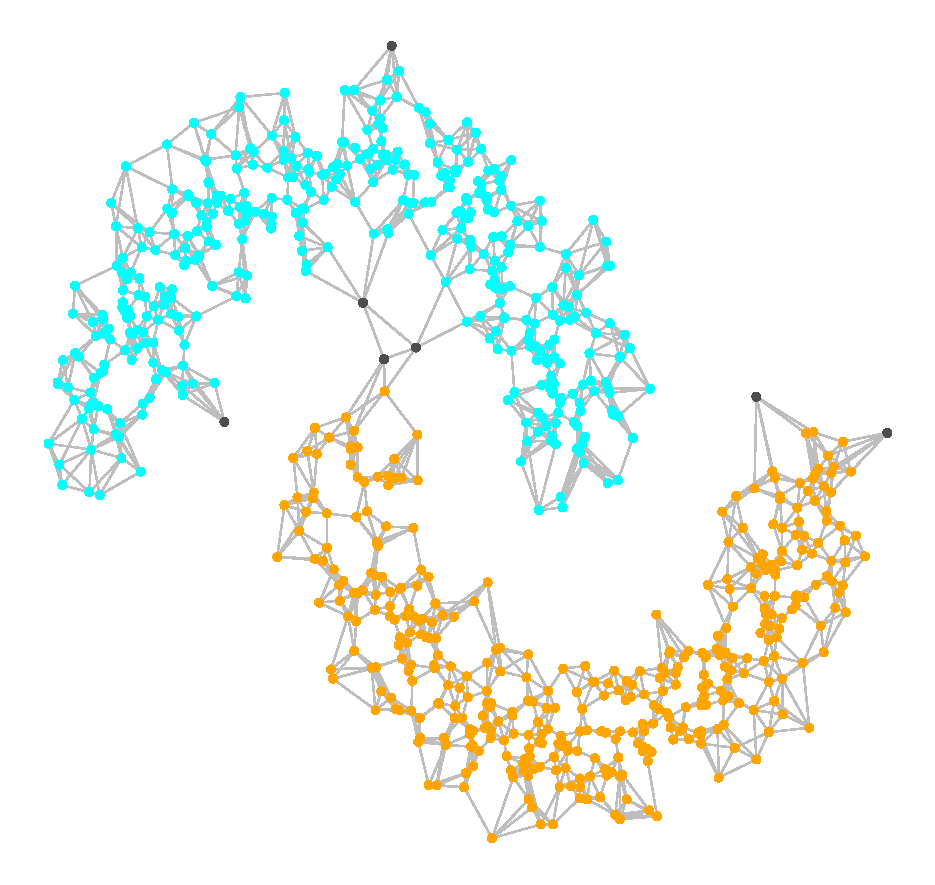
\includegraphics[width=0.24\textwidth,scale = .5]{example2plots/row1_true_density_cluster}
	% \caption{}
	% \end{subfigure}
	% \begin{subfigure}{.24\linewidth}
	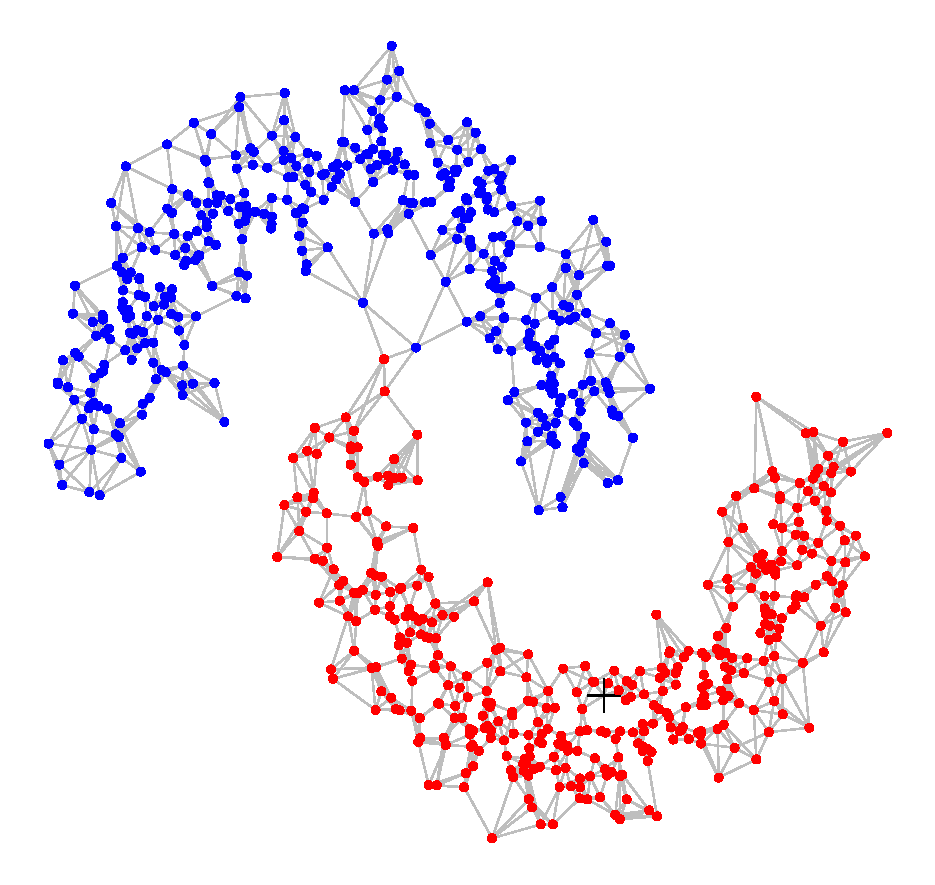
\includegraphics[width=0.24\textwidth]{example2plots/row1_ppr_cluster}
	% \caption{}
	% \end{subfigure}
	% \begin{subfigure}{.24\linewidth}
	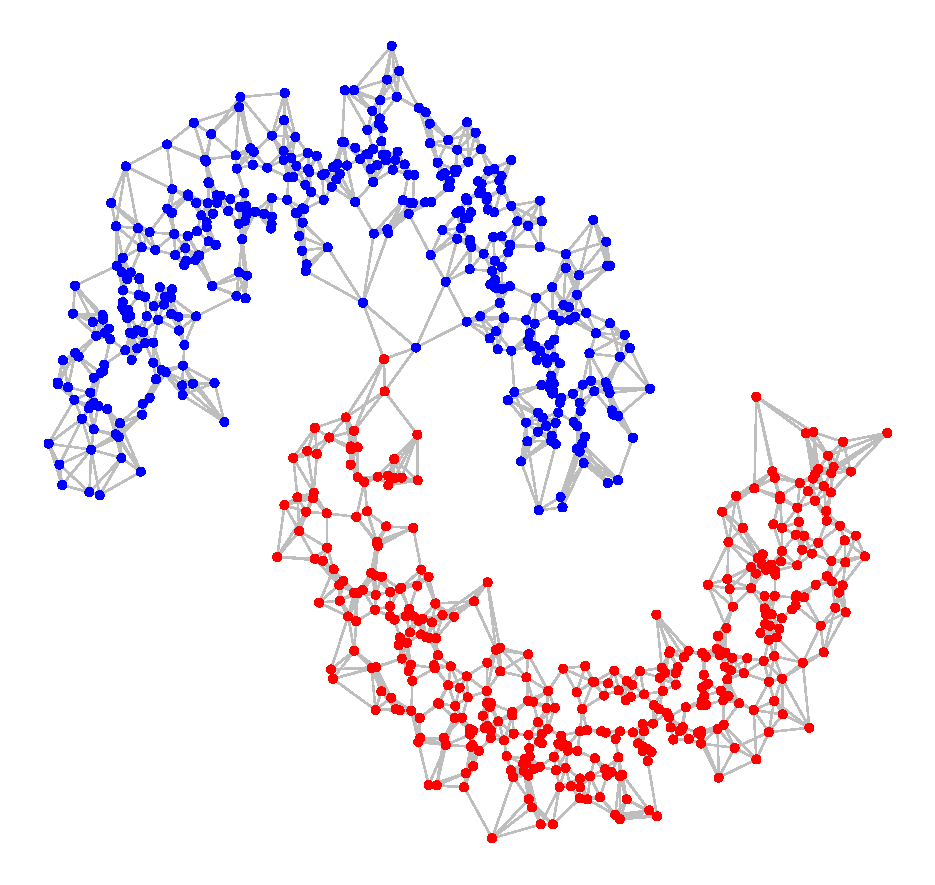
\includegraphics[width=0.24\textwidth]{example2plots/row1_conductance_cluster}
	% \caption{}
	% \end{subfigure}
	% \begin{subfigure}{.24\linewidth}
	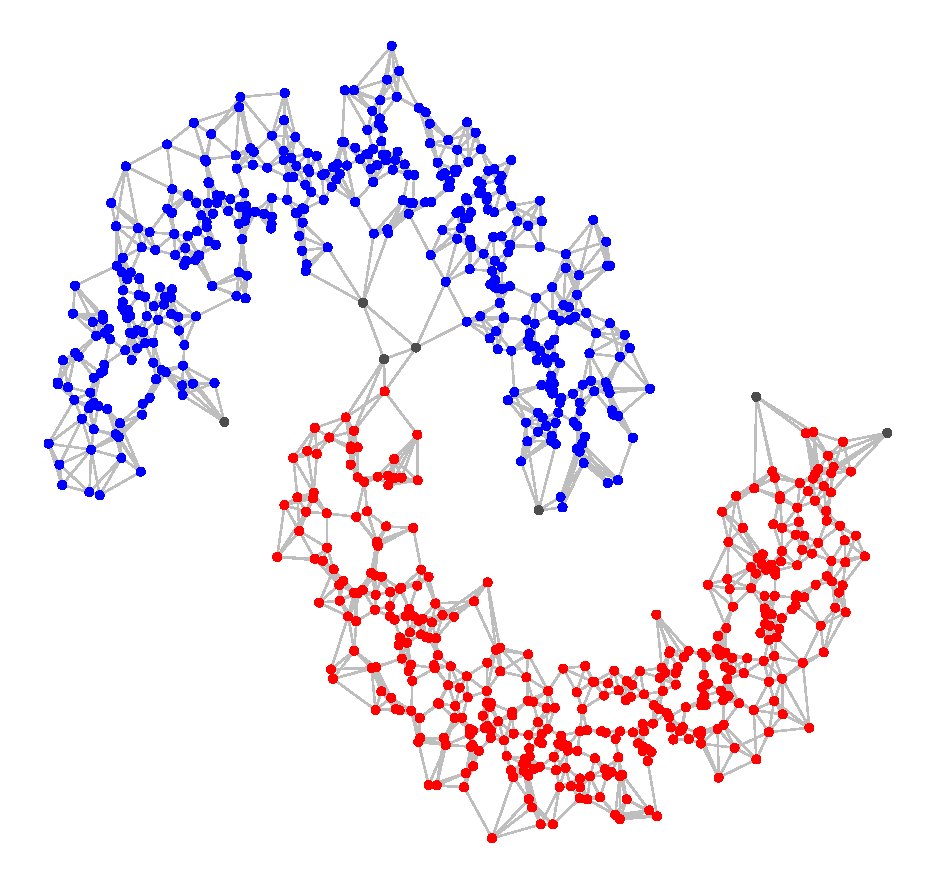
\includegraphics[width=0.24\textwidth]{example2plots/row1_density_cluster}
	% \caption{}
	% \end{subfigure}
	
	% \begin{subfigure}{.24\linewidth}
	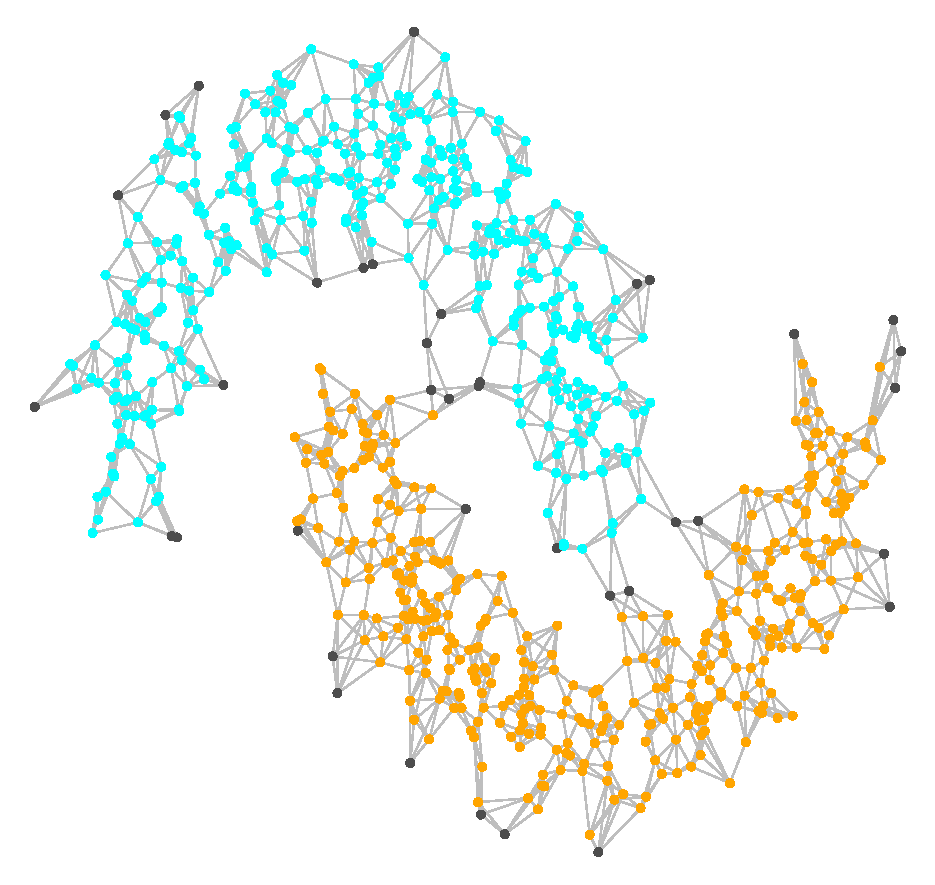
\includegraphics[width=0.24\textwidth]{example2plots/row2_true_density_cluster}
	% \caption{}
	% \end{subfigure}
	% \begin{subfigure}{.24\linewidth}
	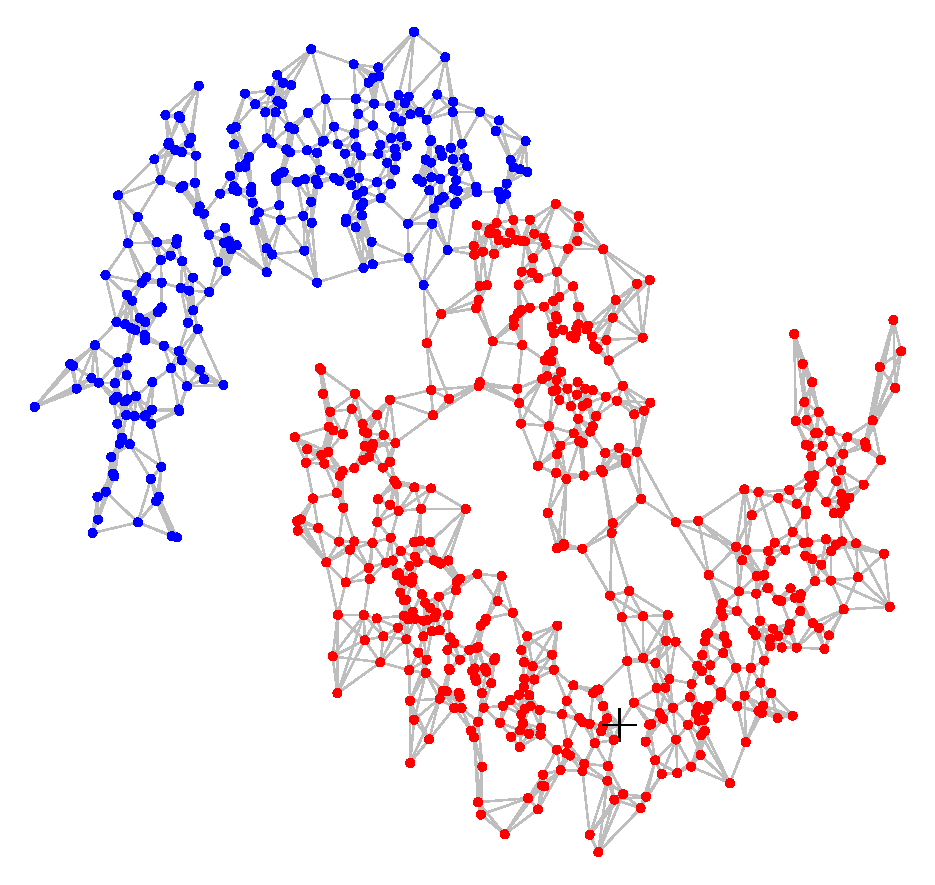
\includegraphics[width=0.24\textwidth]{example2plots/row2_ppr_cluster}
	% \caption{}
	% \end{subfigure}
	% \begin{subfigure}{.24\linewidth}
	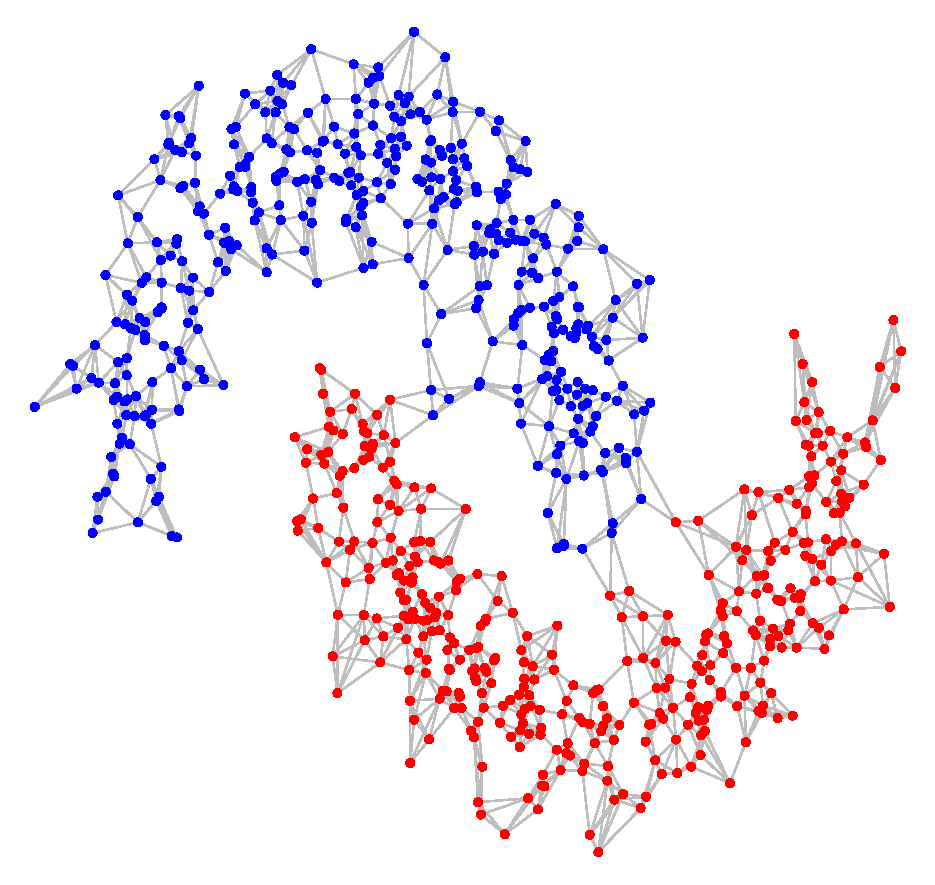
\includegraphics[width=0.24\textwidth]{example2plots/row2_conductance_cluster}
	% \caption{}
	% \end{subfigure}
	% \begin{subfigure}{.24\linewidth}
	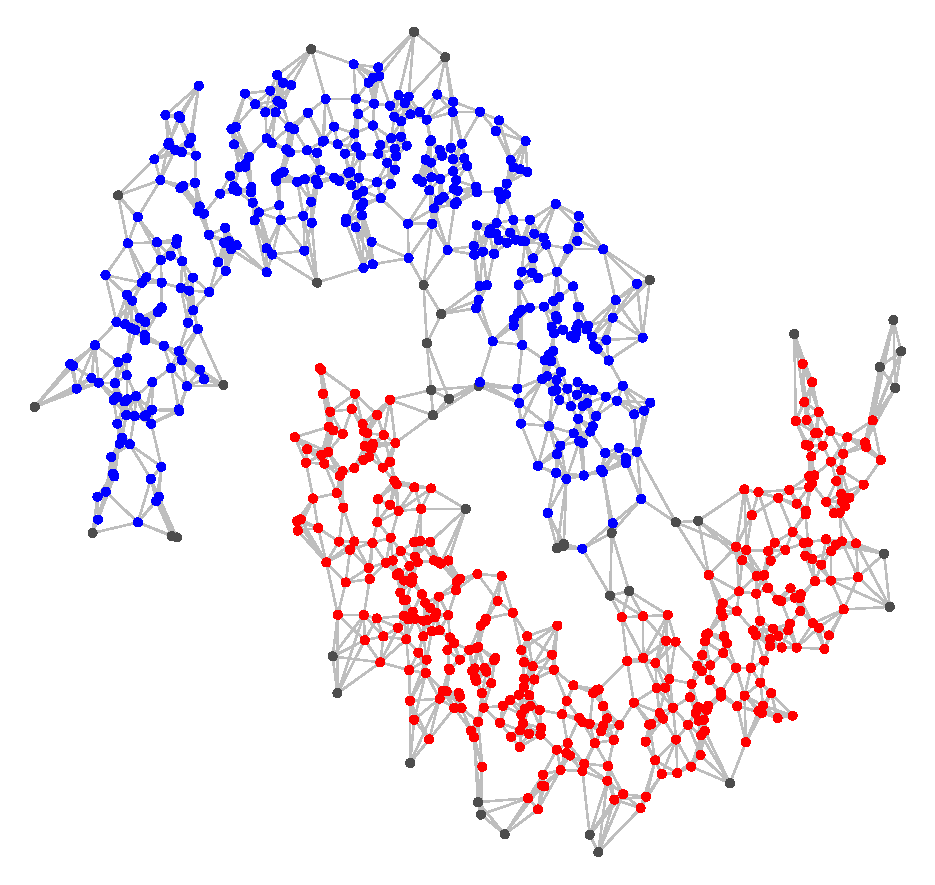
\includegraphics[width=0.24\textwidth]{example2plots/row2_density_cluster}
	% \caption{}
	% \end{subfigure}
	
	% \begin{subfigure}{.24\linewidth}
	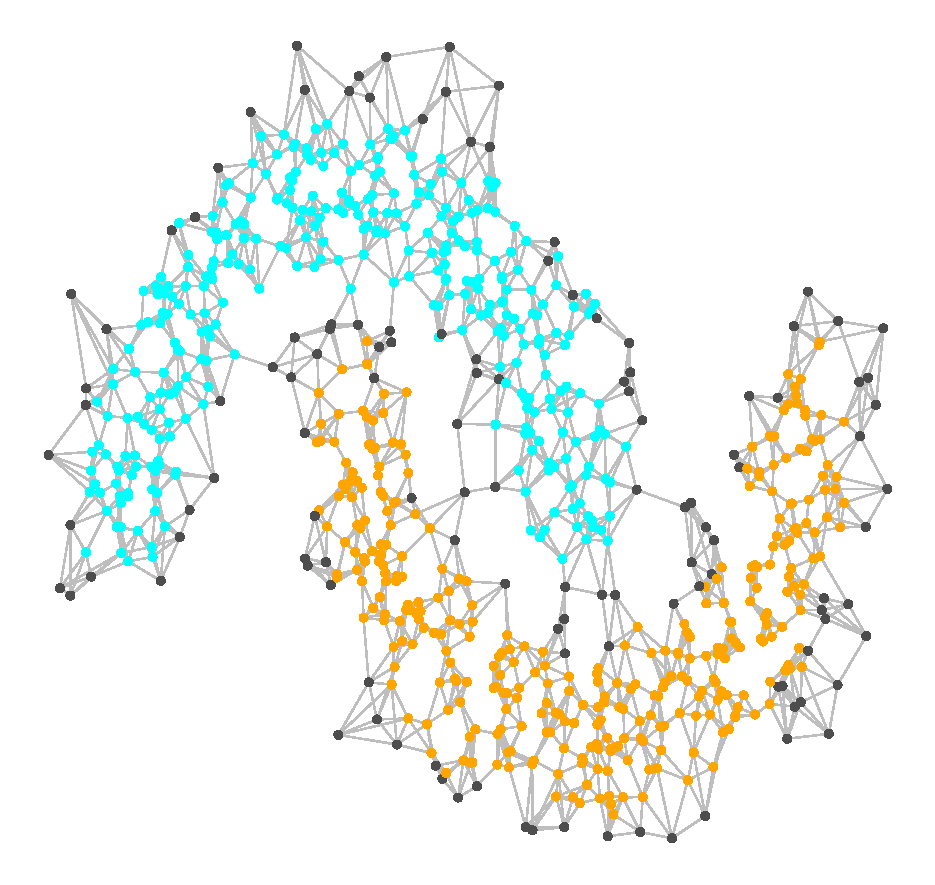
\includegraphics[width=0.24\textwidth]{example2plots/row3_true_density_cluster}
	% \caption{}
	% \end{subfigure}
	% \begin{subfigure}{.24\linewidth}
	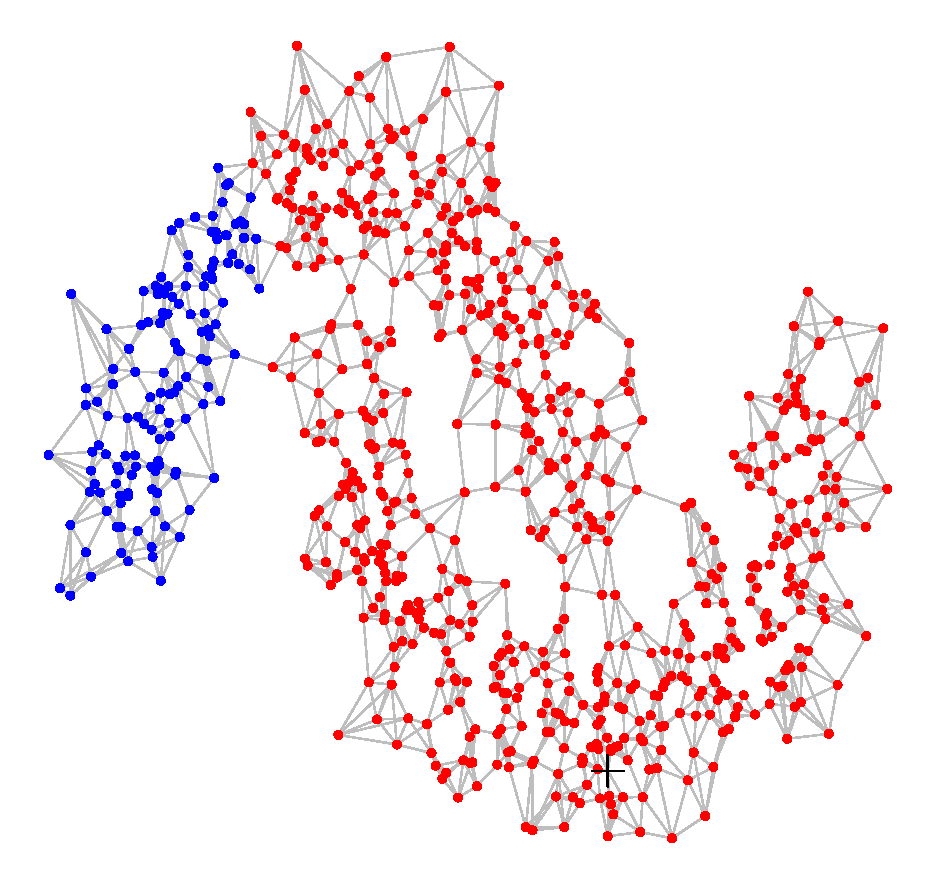
\includegraphics[width=0.24\textwidth]{example2plots/row3_ppr_cluster}
	% \caption{}
	% \end{subfigure}
	% \begin{subfigure}{.24\linewidth}
	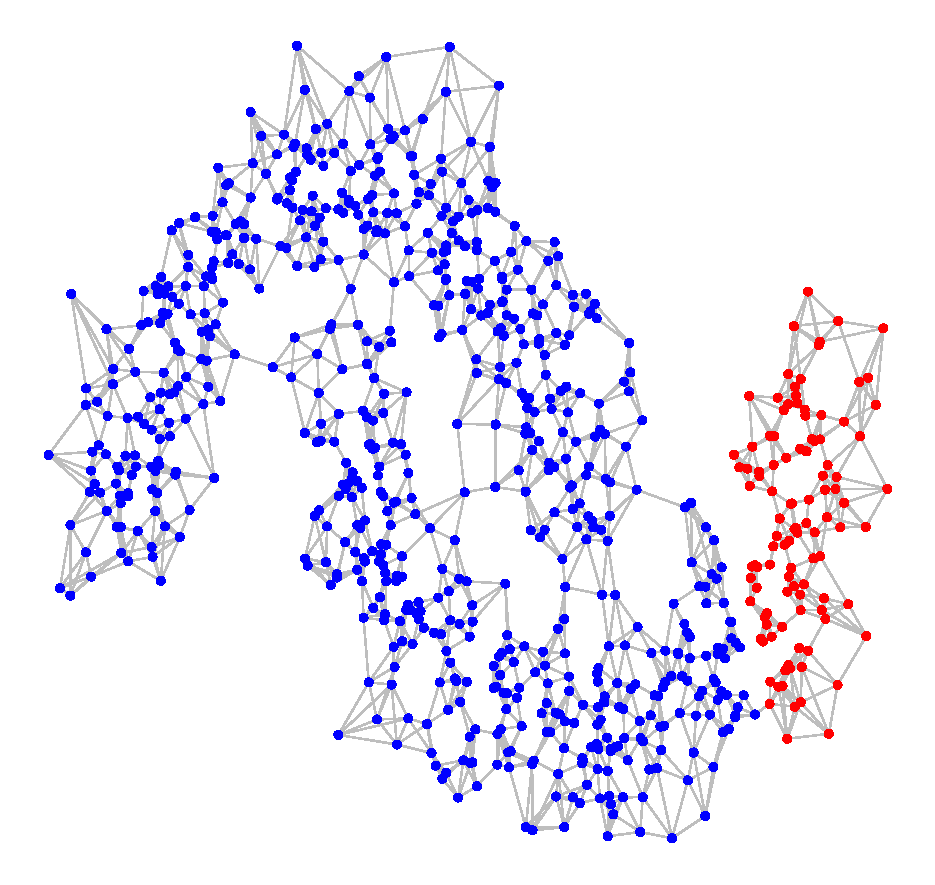
\includegraphics[width=0.24\textwidth]{example2plots/row3_conductance_cluster}
	% \caption{}
	% \end{subfigure}
	% \begin{subfigure}{.24\linewidth}
	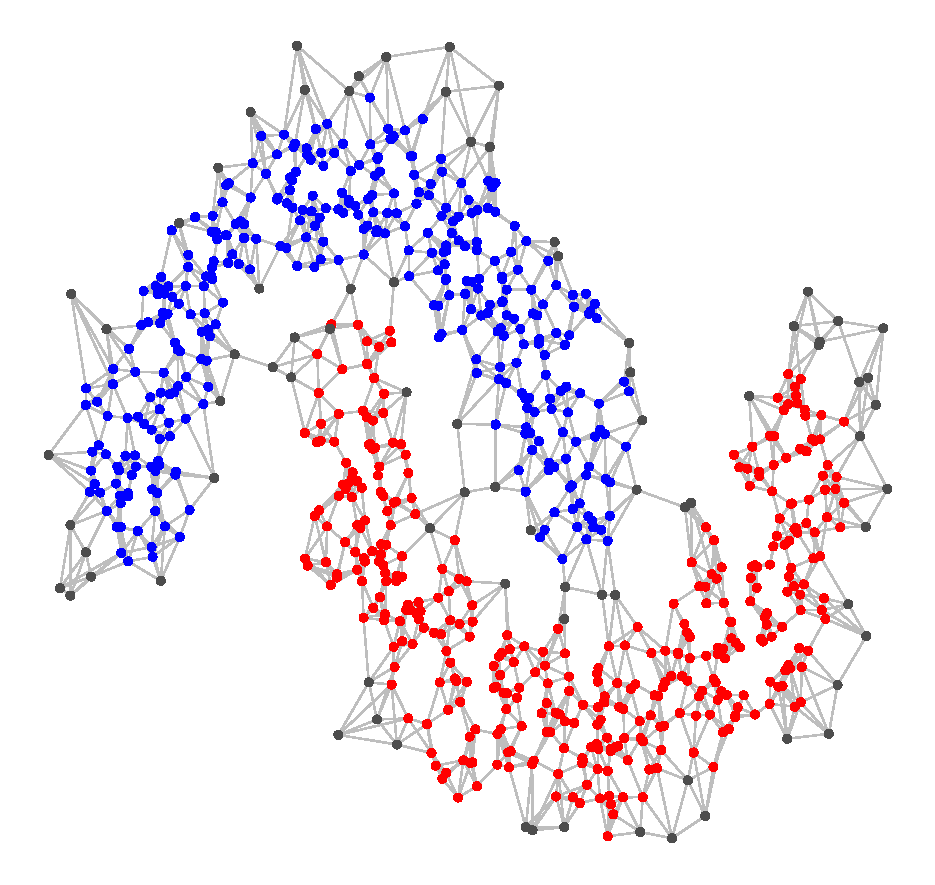
\includegraphics[width=0.24\textwidth]{example2plots/row3_density_cluster}
	% \caption{}
	% \end{subfigure}
	\caption{\it\small True density (column 1), PPR (column 2), normalized
		cut (column 3) and estimated density (column 4) clusters for 3 different 
		simulated data sets. Seed node for PPR denoted by a black cross.} 
	\label{fig:fig2}
	%\end{adjustbox}
\end{figure}

\section{Hypothesis testing with neighborhood graphs.}

We define test statistics for both the regression and density testing setups. In the former, we show in some preliminary work that our proposed test statistic is minimax optimal over the Sobolev ball $W^{1,2}(\mathcal{X};1)$. In the latter, we empirically demonstrate that our proposed approach has merit. We conclude this section by discussing some practical and computational considerations for this problem. Throughout, in subsections entitled ``Proposed Work'' we detail the work we intend to complete for a final thesis. 

\subsection{Regression testing using graph spectral projections.}
\label{subsec:spectral_regression_testing}

Recalling the regression model~\eqref{eqn:regression}, let $VSV^T$ be the spectral decomposition of the Laplacian matrix $L$ of the neighborhood graph $G_{n,r}$. Inspired by \eqref{eqn:harmonic}, we propose the following truncated-series test statistic:
\begin{equation}
\label{eqn:graph_spectral_projections}
T_{\mathrm{spec}} := \frac{1}{n} \sum_{k = 0}^{\kappa} \left(\sum_{i = 1} v_i y_i\right)^2
\end{equation}
where the main difference between $T_{\mathrm{spec}}$ and $T_{\mathrm{harm}}$ is that the eigenvectors $\set{v_i}$ are now playing the role of the harmonic functions $\set{\phi_{\ell}}$. In Theorem~\ref{thm:sobolev_testing_rate} we show that under some mild regularity conditions on $\Pbb$, the test $\phi_{\textrm{spec}} := \1\{T_{\mathrm{spec}} \geq \tau\}$ is, up to log factors, a minimax optimal test over the Sobolev ball $W^{1,2}(\mathcal{X};1)$. To conveniently state our results we introduce the notation
\begin{equation*}
h(\beta,d) = (1/d + \beta)(d/2 + s)(2d/(4s + d))
\end{equation*}

\begin{theorem}
	\label{thm:sobolev_testing_rate}
	Let $b \geq 1,\beta > 0$ be fixed constants and let $d < 4$. Suppose that $\Pbb$ is an absolutely continuous probability measure over $\mathcal{X} = [0,1]^d$ with density function $p$ bounded above and below by constants, i.e
	\begin{equation*}
	0 < p_{\textrm{min}} < p(x) < p_{\textrm{max}} < \infty, \quad \textrm{for all $x \in \mathcal{X}$.}
	\end{equation*}
	Then there exists a constant $c_1(d,L,p_{\max},b,\beta)$ which is independent of the sample size $n$ such that the following statement holds: Construct the test statistic $T_{\mathrm{spec}}$ with parameter choices $r \asymp n^{-1/d}$ and $\kappa \asymp n^{2d/(4+d)}$, and additionally let the threshold $\tau \asymp \frac{\kappa}{n} + b\sqrt{\frac{\kappa}{n^2}}$. Then, for every $\epsilon$ satisfying
	\begin{equation}
	\label{eqn:sobolev_testing_rate}
	\epsilon^2 \geq c_1(d,L,p_{\max},b,\beta) \cdot b \cdot n^{-4/(4 + d)} (\log n)^{h(\beta,d)}
	\end{equation}
	the worst-case risk is lower bounded
	\begin{equation}
	\label{eqn:sobolev_testing_rate_1}
	\mathcal{R}(\phi_{\mathrm{spec}}; \mathcal{W}^{1,2}(\mathcal{X};L)) \leq \left(\frac{2}{b^2} + \frac{2}{b\sqrt{\kappa}}\right) + o(1).
	\end{equation}
	Therefore, $\epsilon_n^2(\phi_{\mathrm{spec}}, \mathcal{W}^{1,2}(\mathcal{X};L)) \asymp  n^{-4/(4 + d)} (\log n)^{h(\beta,d)}$. 
\end{theorem}

A comparison of Theorem~\ref{thm:sobolev_testing_rate} with the rates derived by~\citet{ingster09} for a test based on $T_{\mathrm{harm}}$ demonstrates that the additional error incurred by using estimated eigenfunctions of the Laplacian, rather than directly using the Fourier series, results in the critical radius widening by only at most a factor of $(\log n)^{h(\beta,d)/2}$ from the minimax critical radius over $W^{1,2}(\mathcal{X};1)$. This means our test based on $T_{\textrm{spec}}$ is almost \textit{as good as}, in a minimax sense, the best possible test over $W^{1,2}(\mathcal{X};1)$. As mentioned previously, when $d \geq 4$ the problem  requires different assumptions on $f$ and is characterized by a different minimax rate.

We have shown that the test $\phi_{\mathrm{spec}}$ has some desirable theoretical properties. However, more comprehensive theoretical work is required to fully motivate $\phi_{\mathrm{spec}}$, and to better characterize its performance.

\subsubsection{Proposed work.}

Theorem~\ref{thm:sobolev_testing_rate} shows that the test $\phi_{\mathrm{spec}}$ is nearly-minimax optimal over $W_d^{1,2}(\mathcal{X};L)$. We propose to study the minimax properties of $\phi_{\mathrm{spec}}$ over two related Sobolev spaces, (i) the higher-order Sobolev balls $W_d^{s,2}(\mathcal{X};L)$, and (ii) density-weighted versions of Sobolev spaces.

\paragraph{Higher-order Sobolev spaces.}
In order to extend our results to hold with respect to the balls $W_d^{s,2}(\mathcal{X};L)$, we will likely need to consider kernels $K_r(u,v) = K\left(\frac{\norm{u - v}}{r}\right)$ for which
\begin{equation}
\label{eqn:higher_order_kernel}
\int x^i K(x) \,dx = 0, \quad \textrm{i = 1,\ldots,s}
\end{equation}
as is typical in nonparametric smoothing problems \cite{tsybakov08}. Choosing kernels which satisfy~\eqref{eqn:higher_order_kernel}--as opposed to our current choice of kernel $K_r(x,y) = \1(\norm{x - y} \leq r)$--allows for tighter control on the quadratic functional
\begin{equation*}
\int \int (f(x) - f(y))^2 K_r(x,y) \,d\Pbb(x) \,d\Pbb(y);
\end{equation*}
this control is critical to obtain minimax rates, and otherwise the analysis when $s = 1$ versus $s > 1$ is not substantially different. We therefore \textbf{intend} to show for any Sobolev ball $W_d^{s,2}(\mathcal{X};L)$ such that $4s > d$, if the kernel $K$ satisfies~\eqref{eqn:higher_order_kernel} and the tuning parameters $\kappa$ and $r$ are selected appropriately, the test $\phi_{\mathrm{spec}}$ is minimax optimal.

\paragraph{Weighted Sobolev norms.}

The aforementioned completed and proposed work shows/would show that our test $\phi_{\mathrm{spec}}$ has minimax properties as good as any other minimax optimal test; for instance, a test based on the statistic $T_{\mathrm{harm}}$ defined in~\eqref{eqn:harmonic}. However, we would like to argue that in certain cases, $T_{\textrm{spec}}$ is in fact \textit{better} than competitors such as $T_{\textrm{harm}}$. We know from results in Section~\ref{subsec:neighborhood_graphs_spectra} that the eigenvectors $\set{v_i}$ converge towards eigenfunctions of a \emph{weighted} Laplacian operator. At a high-level, these eigenfunctions display inhomogeneous smoothness as a function of density, appearing much more wiggly in regions of low-density. 

The behavior of these eigenfunctions should affect the performance of $T_{\mathrm{spec}}$ in predictable ways.  In particular, the test statistic $T_{\mathrm{spec}}$ should be more sensitive than $T_{\mathrm{harm}}$ and other test statistics which perform more classical smoothing to functions $f$ which have smooth deviations from $f_0 = 0$ in high-density regions, but are potentially much wigglier in low-density regions. We will therefore consider the performance of our test $\phi_{\mathrm{spec}}$ over the unit ball in a weighted Sobolev norm 
\begin{equation*}
\mathcal{W}_d^{1,2}(\mathbb{P};\mathcal{X};L) := \set{f \in L^2(\mathcal{X}): \sum_{\abs{\alpha} \leq s}\int\ \int_{\mathcal{X}} \abs{D^{\alpha}f(x)}^2 p^2(x)\,dx \leq 1}.
\end{equation*}
We \textbf{intend} to upper bound the critical radius $\epsilon_n(\phi_{\mathrm{spec}};\mathcal{W}_d^{1,2}(\mathbb{P};\mathcal{X};L))$ as a function of $\mathbb{P}$ as well as $d$ and $n$, and exhibit choices of $\mathbb{P}$ for which $\phi_{\mathrm{spec}}$ will provably outperform competitors such as tests based on $T_{\mathrm{harm}}$ in the sense of having smaller worst-case risk. (See Figure~\ref{fig:fig3} for some empirical examples in the two-sample density testing case).

\subsection{Density testing using graph spectral projections.}
\label{subsec:spectral_density_testing}

It is straightforward to adapt the test statistic $T_{\mathrm{spec}}$ to the two-sample testing problem. Concatenate the samples in $X = (z_1,\ldots,z_N,y_1,\ldots,y_M)$, and let $a = (\underbrace{N^{-1},\ldots,{N^{-1}}}_{\textrm{length } N},\underbrace{-M^{-1},\ldots,-M^{-1}}_{\textrm{length } M})$ encode whether a sample in $X$ comes from $Z$ or $Y$. Letting $n = N + M$, we define the variant $T_{\mathrm{spec}}^{(2)}$ of $T_{\mathrm{spec}}$ to be
\begin{equation}
\label{eqn:graph_spectral_projections_2}
T_{\mathrm{spec}}^{(2)} := \frac{1}{n} \sum_{k = 0}^{\kappa} \left(\sum_{i = 1}^{n} v_i a_i\right)^2
\end{equation}
where as before $v_1,\ldots,v_n$ are eigenvectors of the Laplacian $L = L(X,r)$. Figure~\ref{fig:fig3} shows some instances in which $T_{\mathrm{spec}}^{(2)}$ outperforms a range of common nonparametric tests. We see that the examples support our intuition; $T_{\textrm{spec}}^{(2)}$ is especially strong when the difference in densities $p - q$ oscillates at a higher frequency in regions where the mixture density $\frac{1}{2}(p + q)$ is small. While these examples empirically motivate the use of $T_{\mathrm{spec}}^{(2)}$, at present we still lack a proper theoretical characterization of its performance. This is what we propose to study. 

\begin{figure}
	\label{fig:fig3}
	\centering
	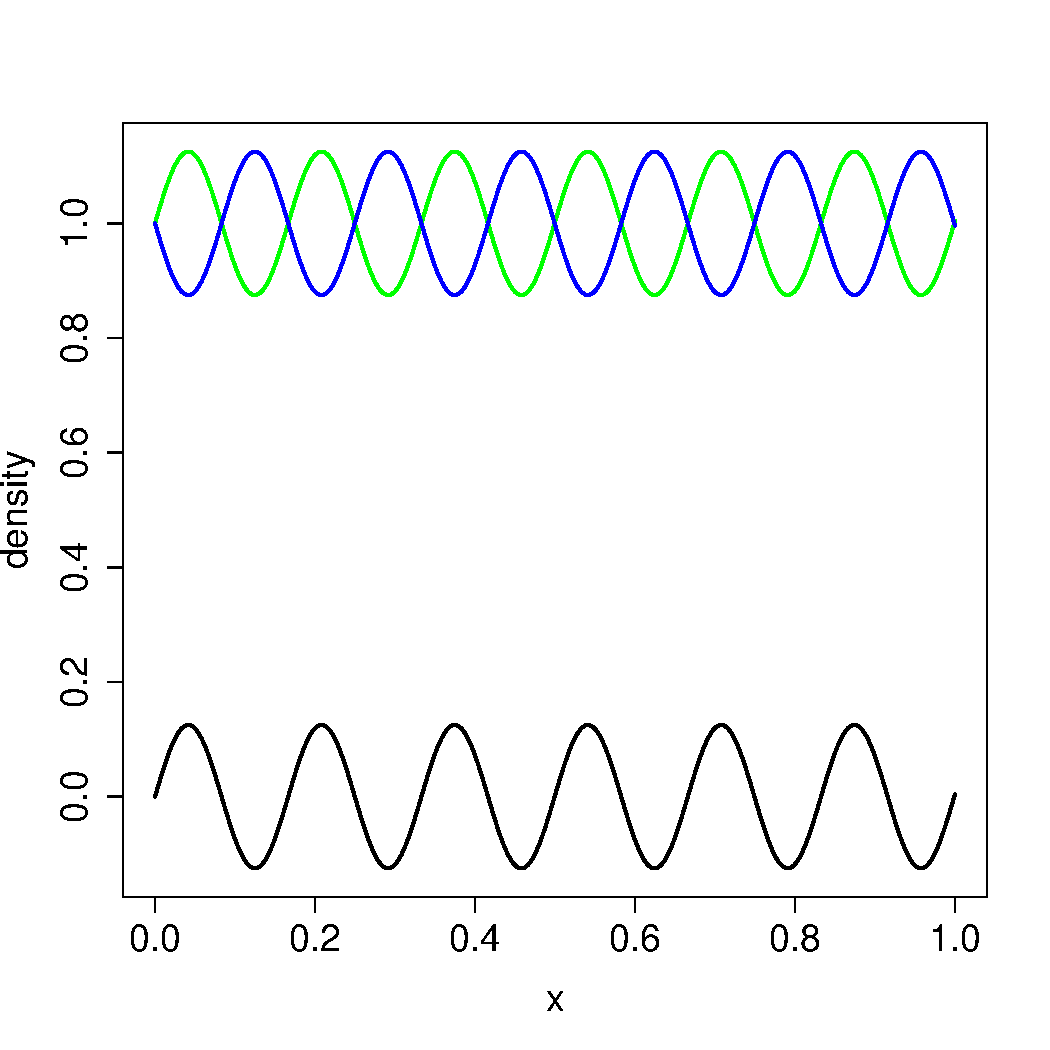
\includegraphics[width=0.32\textwidth]{plots/sin_density}
	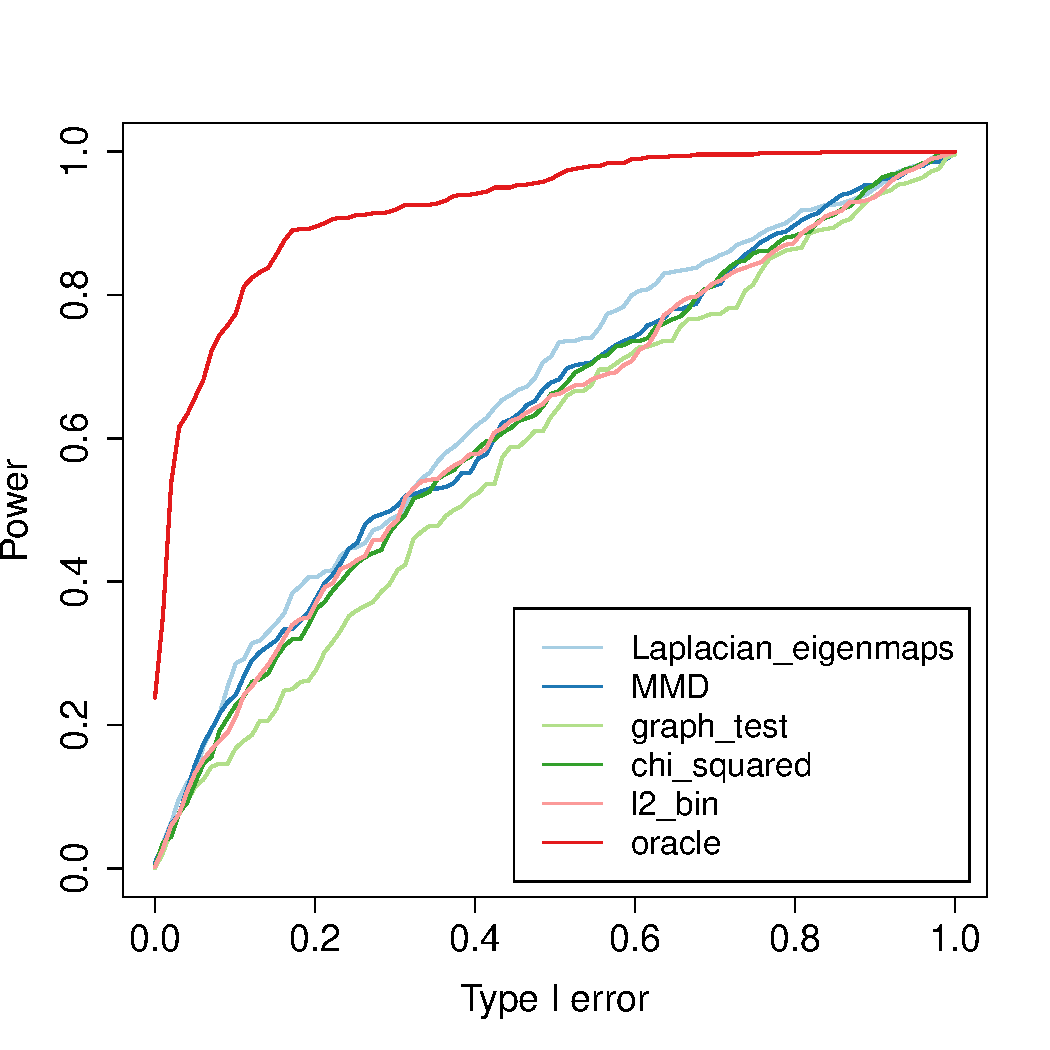
\includegraphics[width=0.32\textwidth]{plots/sin_ROC}
	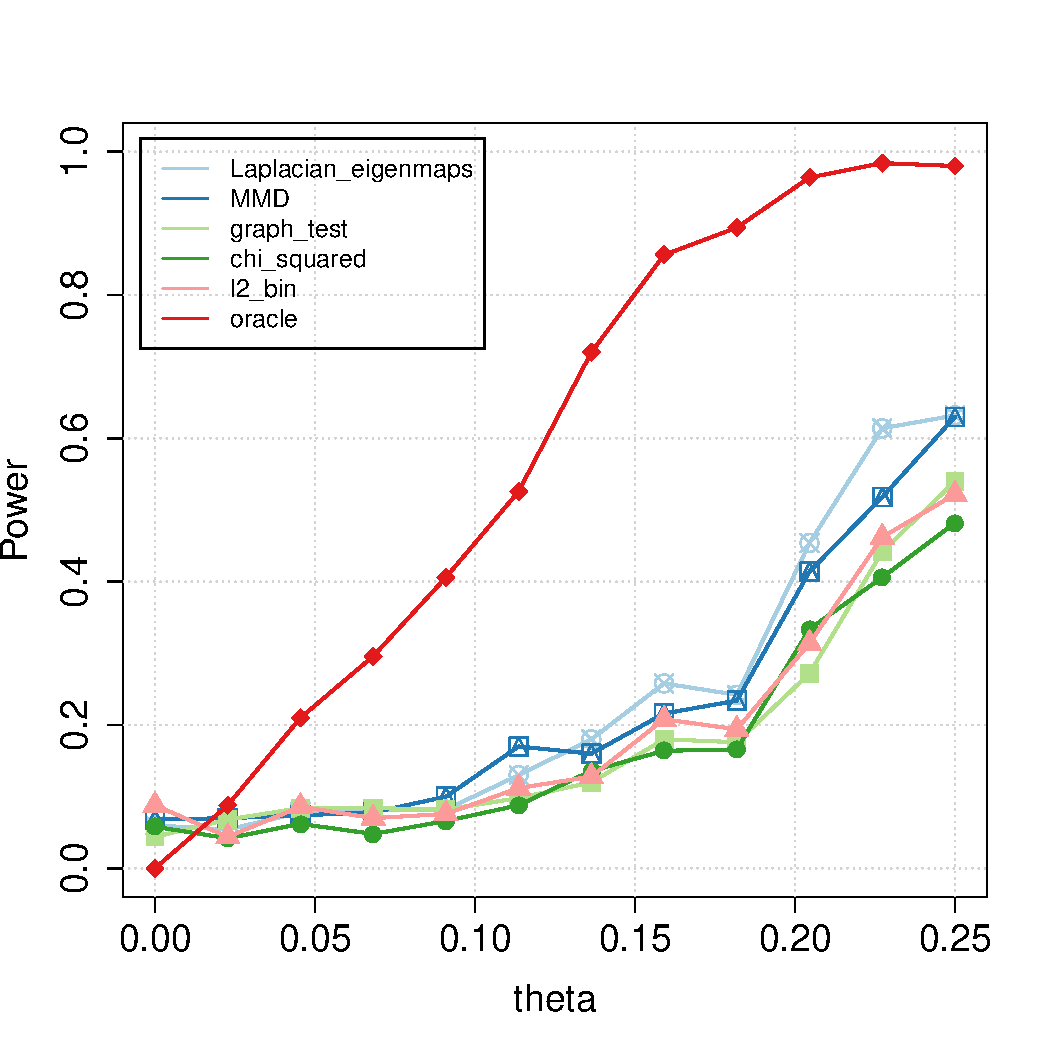
\includegraphics[width=0.32\textwidth]{plots/sin_theta}
	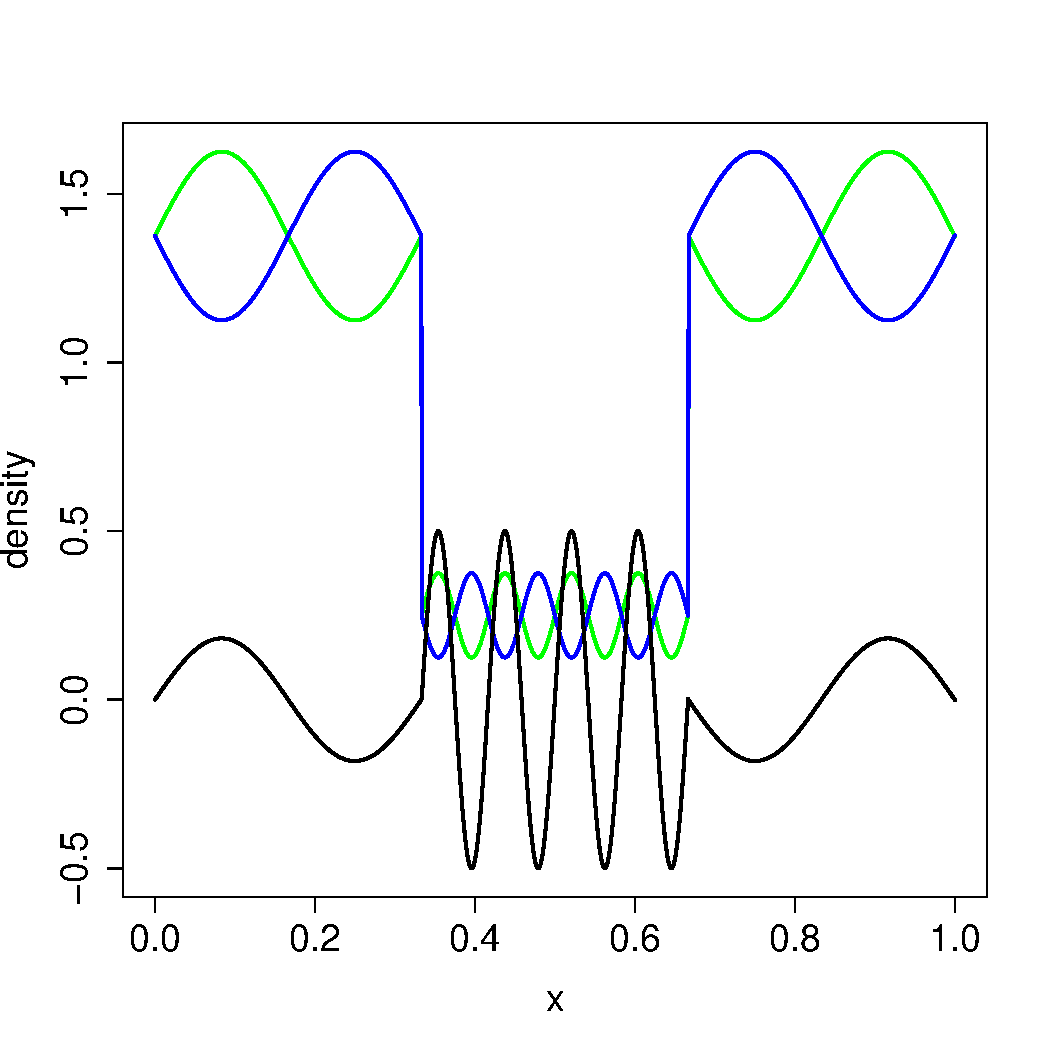
\includegraphics[width=0.32\textwidth]{plots/stepfunction_sin_density}
	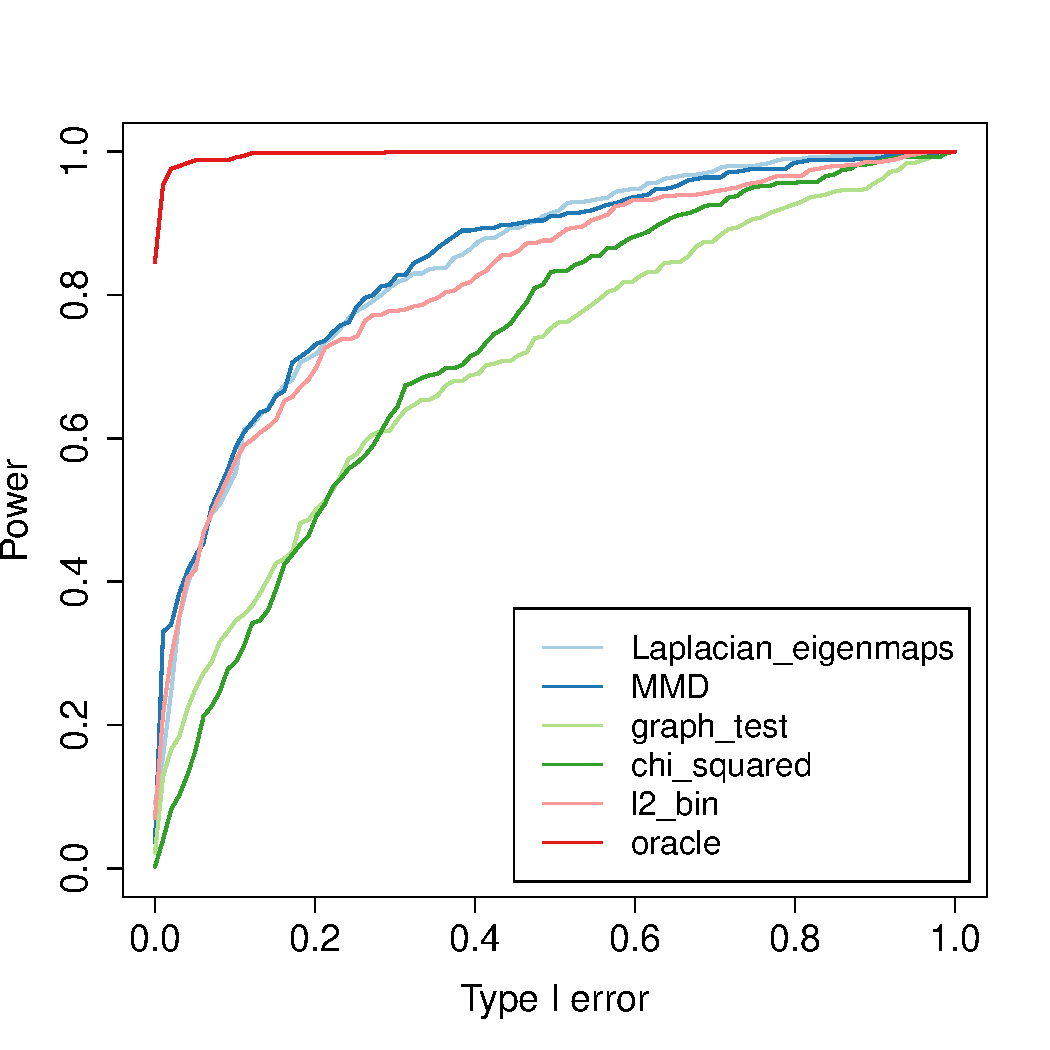
\includegraphics[width=0.32\textwidth]{plots/stepfunction_sin_ROC}
	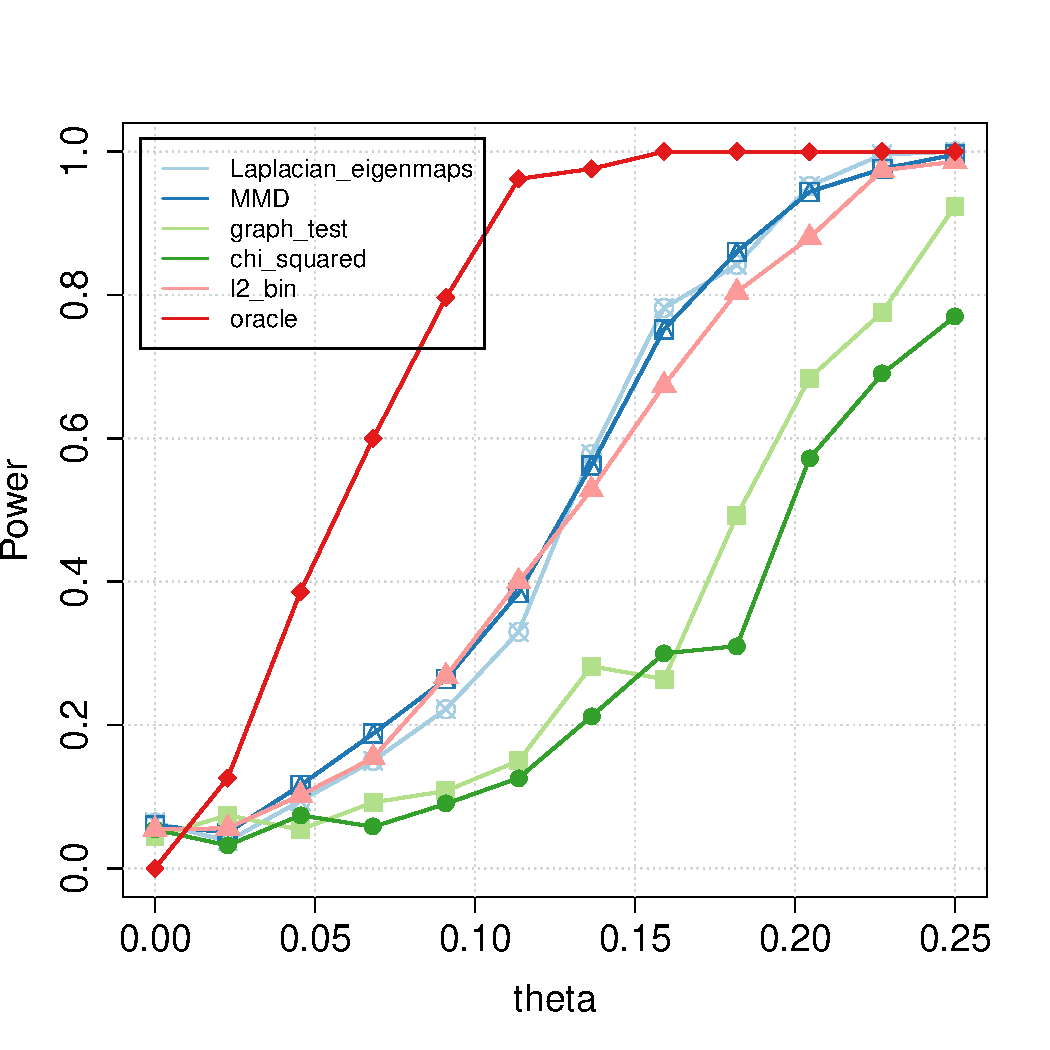
\includegraphics[width=0.32\textwidth]{plots/stepfunction_sin_theta}
	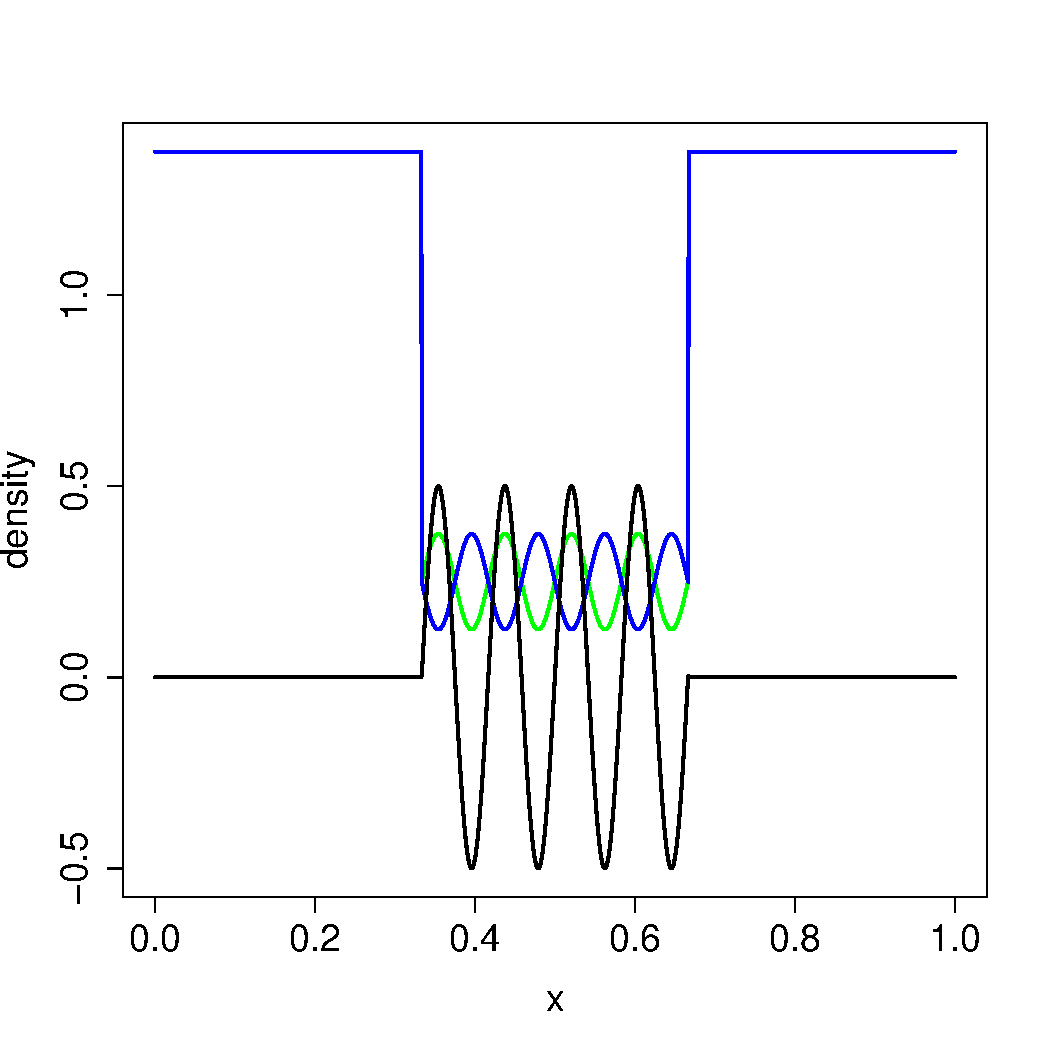
\includegraphics[width=0.32\textwidth]{plots/stepfunction_sin2_density}
	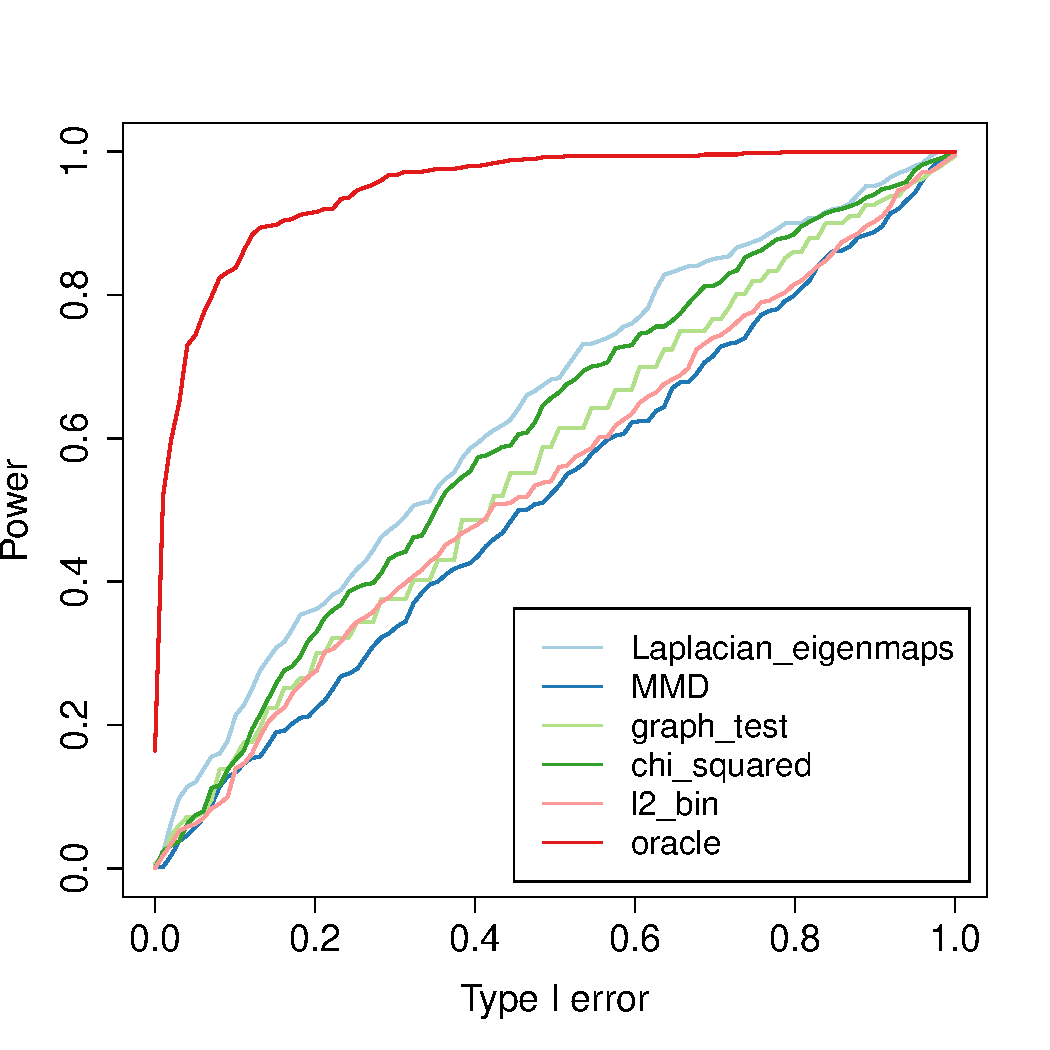
\includegraphics[width=0.32\textwidth]{plots/stepfunction_sin2_ROC}
	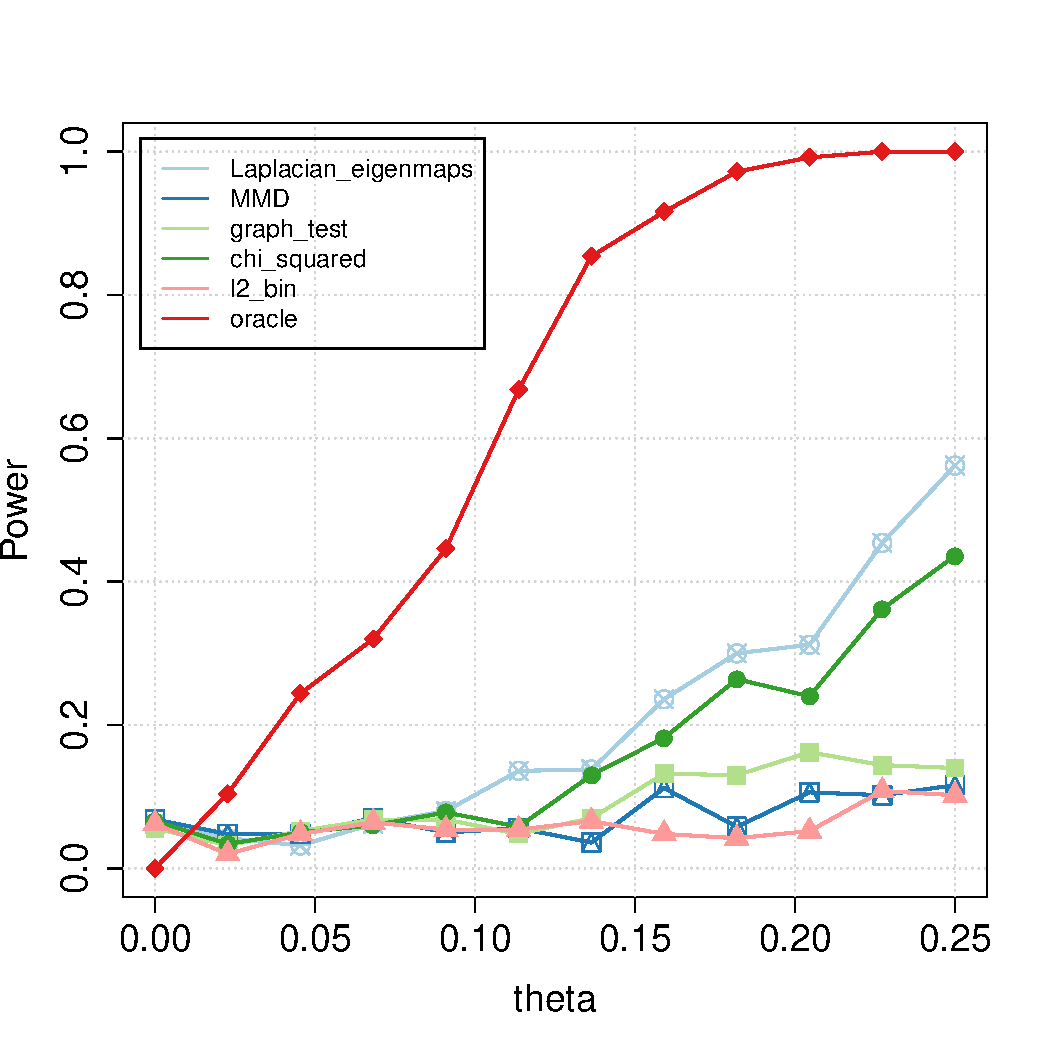
\includegraphics[width=0.32\textwidth]{plots/stepfunction_sin2_theta}
	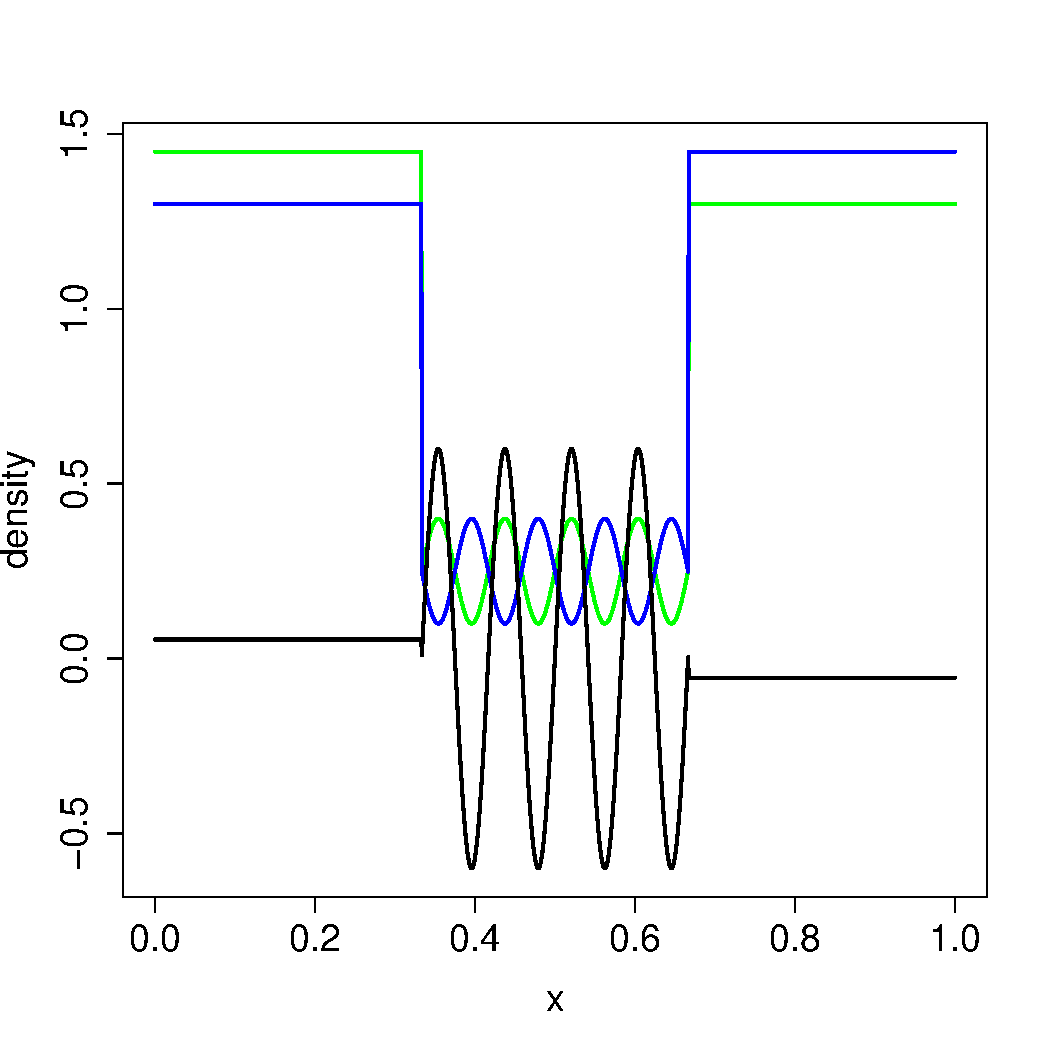
\includegraphics[width=0.32\textwidth]{plots/stepfunction_sin3_density}
	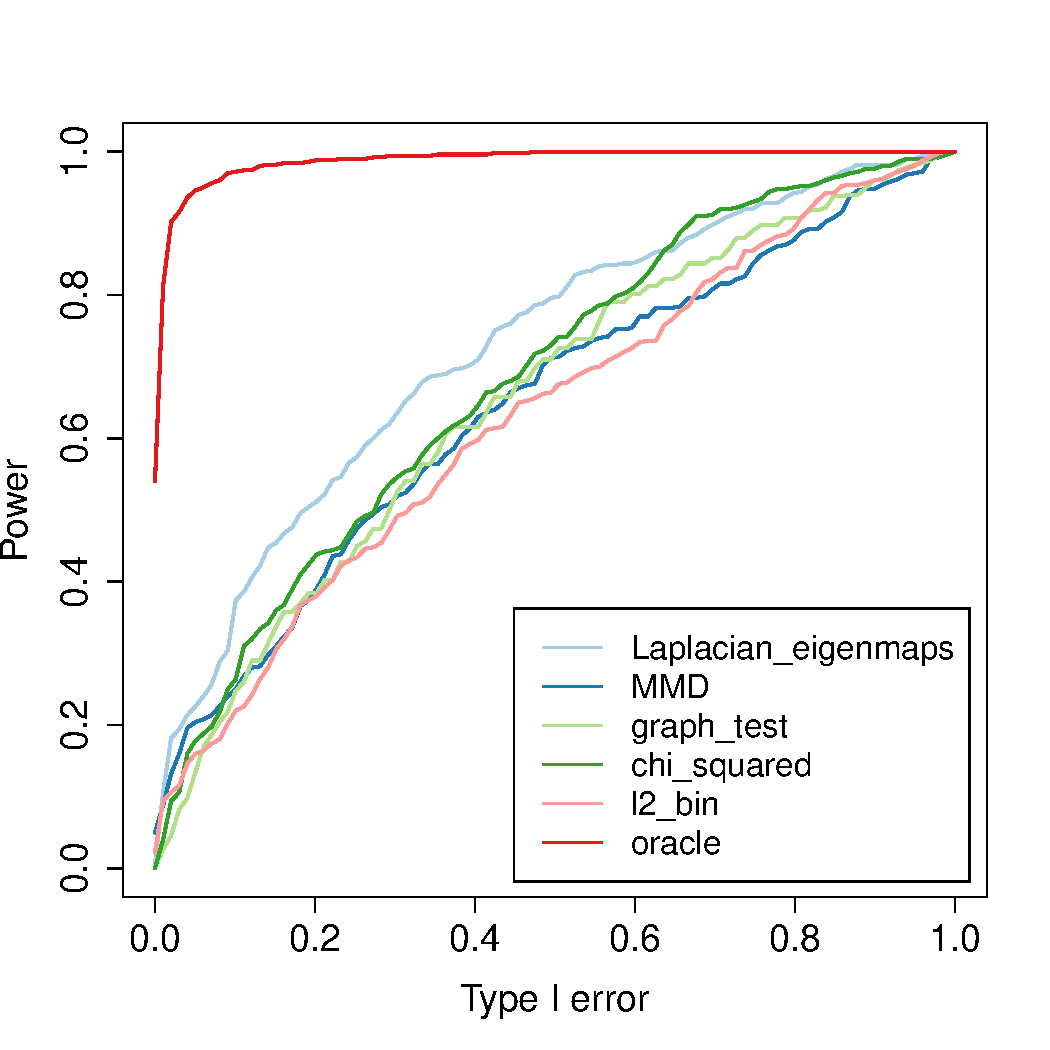
\includegraphics[width=0.32\textwidth]{plots/stepfunction_sin3_ROC}
	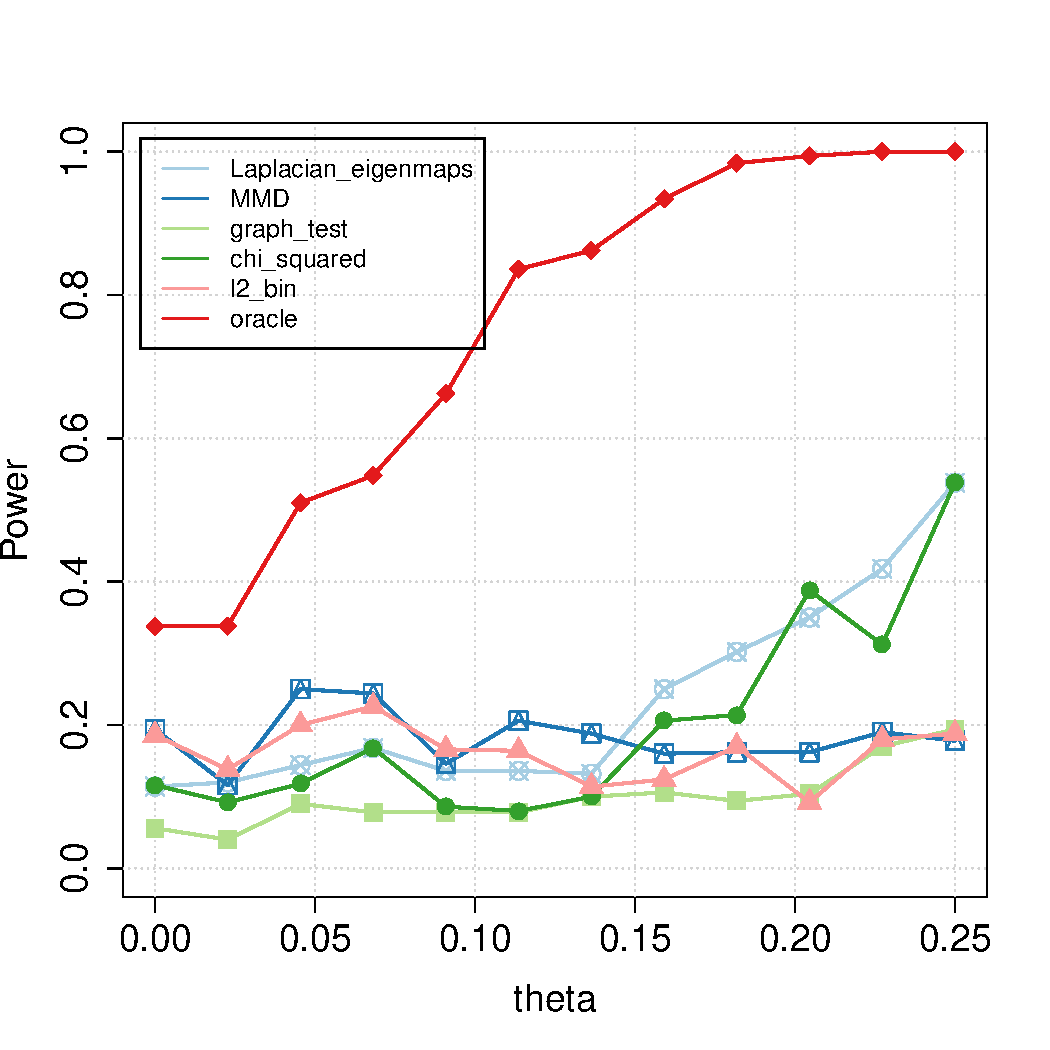
\includegraphics[width=0.32\textwidth]{plots/stepfunction_sin3_theta}
\end{figure}

\subsubsection{Proposed work.}

As previously mentioned the minimax critical radius for the two-sample density testing problem over $C_d^{s}(\mathcal{X};L)$ is known to be $\epsilon_n^{\star}(C_d^{s}(\mathcal{X};L)) \asymp n^{-2s/(4s + d)}$ for all $d \geq 1$ and $s > 0$. Letting $\phi_{\mathrm{spec}}^{(2)} := \1\{T_{\mathrm{spec}} > \tau\}$, we \textbf{intend} to show that the critical radius $\epsilon_n(\phi_{\mathrm{spec}}^{(2)};C_d^{s}(\mathcal{X};L)) \asymp n^{-2s/(4s + d)}$ for all $d \geq 1, s > 0$, thus establishing that the test is minimax optimal over $C_d^{s}(\mathcal{X};L)$.

There are certain technical nuances which make studying $T_{\mathrm{spec}}^{(2)}$ in the density testing problem more subtle than studying $T_{\mathrm{spec}}$ in the regression testing problem. (In particular, we require a condition on convergence of the eigenvectors ${v_i}$ which presently eludes us.) However, besides this issue by and large the technical results required are the same in each problem \emph{when the condition $4s > d$ is met}.

\paragraph{Density testing for irregular ($4s \leq d$) alternatives.}

% As mentioned in Section~\ref{subsubsec:density_testing}, the regression and density testing models over e.g. Holder spaces are formally asymptotically equivalent; however, these asymptotic equivalence statements hold only when $2s > d$. To illuminate some differences between the density and regression testing problems when the regression function $f$ or difference in densities $p - q$ is considered to be irregular (meaning $2s < d$), it is helpful to consider the following generative model: suppose we observe pairs $(x_i,\ell_i)$ for $i = 1,\ldots, (n + m)$, where as usual $x_i \sim \Pbb$ are independent, and additionally $\ell_i$ are conditionally independent given $x_i$ with distribution
%\begin{equation*}
%\begin{cases*}
%1, & ~~  \textrm{with probability $\frac{p(x)}{p(x) + q(x)}$} \\
%-1, & ~~ \textrm{with probability $\frac{q(x)}{p(x) + q(x)}$.} 
%\end{cases*}
%\end{equation*}
%We can relate this to the density testing problem by applying Bayes rule, whence we derive that the conditional distribution of $X_i|\ell_i = 1$ is $\mathbb{P}$, and similarly the conditional distribution of $X_i|\ell_i = -1$ is $\mathbb{Q}$. On the other hand, since $\ell_i = f(x_i) + w_i$ where $f = \frac{p - q}{p + q}$ and $w_i$ is a mean-zero error term, this resembles in some respects the regression testing setup. However, $w_i$ is now heteroskedastic with variance depending on the unknown densities $p$ and $q$. The fact that the variance of $w_i$ is unknown is crucial, and as previously mentioned it implies that there will no longer be a elbow in rates at $d = 4$. Indeed,

Before precisely stating what we intend to show regarding $T_{\mathrm{spec}}^{(2)}$ when $4s \leq d$, it is worth emphasizing the differences between the density testing and regression testing problems when $4s \leq d$. In particular, in the density testing problem, the minimax critical radius is $\epsilon_n^{\star}(C_d^{s}(\mathcal{X};L)) \asymp n^{-2s/(4s + d)}$ for all $d \geq 1$ and $s > 0$. By contrast, the following series of inclusions:
\begin{equation*}
C_d^{s}(\mathcal{X};L) \subseteq \{f: \sup_{x \in \mathcal{X}}\abs{f(x)}\} \subseteq \{f: \norm{f}_{\mathcal{L}^4} \leq L\}
\end{equation*}
and the aforementioned work of \citet{guerre02} show that in the regression testing problem, the minimax critical radius is $\epsilon_n^{\star}(C_d^{s}(\mathcal{X};L)) = O(n^{-1/4})$. 

The upper bounds on the minimax critical radius in the density testing problem can be proved using binning tests, or tests based on truncated series test statistics such as $T_{\mathrm{harm}}$. These latter statistics--which take empirical evaluations of an orthonormal basis in $\mathcal{L}^2(\mathcal{X})$--are minimax optimal over $C_d^{1}(\mathcal{X};L)$ when the number of basis functions is chosen to be $\kappa \asymp n^{2d/(4s+d)}$, meaning $\kappa > n$ when $4s < d$. Since we have only $n$ eigenvectors $v_1,\ldots,v_n$, there is no clear relationship between $T_{\mathrm{harm}}$ and $T_{\mathrm{spec}}^{(2)}$ in this setting.

We will therefore need a new approach to choosing $r$ and $\kappa$ if we want our test $\phi_{\mathrm{spec}}^{(2)}$ to be minimax optimal when $4s \leq d$. Intuition from binning tests--where the optimal choice of bin-width is on the order of $n^{-2s/(4s+d)}$, less than $n^{-1/d}$ whenever $4s < d$--suggests that we should modify our test statistic by choosing $r$ to be shrinking at a rate faster than $n^{-\frac{1}{d}}$. Of course at this connectivity scale with high probability the graph $G_{n,r}$ is disconnected \cite{penrose99}, and our analysis will necessarily be quite different than before. We \textbf{intend} to study the behavior of the graph $G_{n,r}$ when $r = o(n^{-1/d})$, with the hopes of showing that for $r \asymp n^{-2s/(4s+d)}$ and appropriate choices of $\kappa$ and $\tau$, the test $\phi_{\mathrm{spec}}^{(2)}$ has critical radius $\epsilon_n(\phi_{\mathrm{spec}}^{(2)}; C_d^{s}(\mathcal{X};L)) \asymp n^{-2s/(4s + d)}$ even when $4s \leq d$.

\subsection{IPMs on neighborhood graphs.}
\label{sec:neighborhood_graph_IPMs}

In this section, we introduce a pair of graph-based test statistics on the neighborhood graph $G_{n,r}$, which we cast as IPMs over different ``function'' classes $\Theta \subset \Reals^n$. We have not substantively investigated the behavior of these test statistics yet, and therefore we have several lines of proposed work.

\subsubsection{Proposed work: Sobolev IPM on a neighborhood graph.}

We call our first proposed test statistic the \emph{graph Sobolev} IPM, since the function class $\Theta$ over which we take the supremum will resemble a continuous Sobolev space. Formally, we introduce the scaling $C_n := nr^{(d + 2)/2}$, and let
\begin{equation}
\label{eqn:sobolev_IPM}
T_{\textrm{sob}} := \sup_{\theta \in \Theta_{1,2}(\lambda)} \abs{\frac{1}{n}\sum_{i = 1}^{n} a_i \theta_i}, \quad  \Theta_{1,2}(\lambda) := \{\theta \in \Reals^n:~ C_n^{-1} \norm{B\theta}_2 + \frac{\lambda}{n^{1/2}}\norm{\theta}_2 \leq 1\} ~~ \lambda > 0, 
\end{equation}
where we recall $B$ is the incidence matrix of $G_{n,r}$, and the notation $a = \left(N^{-1},\ldots,N^{-1},-M^{-1},\ldots,-M^{-1}\right)$. (We could easily adapt this statistic to the regression testing case by replacing $a$ with $y$, although we would lose the analogy to an IPM).  Several aspects of the statistic $T_{\textrm{sob}}$ are worthy of comment. 

\textbf{Remark:}~~The scalings $C_n$ and $n^{-1/2}$ in front of $\norm{B\theta}_2$ and $\norm{\theta}_2$ are the proper scalings at which to compare these norms to the continuum norms $\norm{\cdot}_{W_d^{s,2}(\mathcal{X})}$ and $\norm{\cdot}_{\mathcal{L}^2(\mathcal{X})}$. These scalings are strictly for convenience, as we could always absorb them into the parameter $\lambda$.  

\textbf{Remark:} The role played by the term $\frac{\lambda}{n^{1/2}}\norm{\theta}_2$ is at first glance somewhat mysterious. It may seem more natural to consider the statistic
\begin{equation*}
\sup_{\theta \in \Reals^n: C_n^{-1}\norm{B\theta}_2 \leq 1} \abs{\frac{1}{n}\sum_{i = 1}^{n} a_i \theta_i}, 
\end{equation*}
so that the function class is defined only with respect to the semi-norm $\norm{B\theta}_2$. However, we have shown in preliminary calculations that this function class is too rich, and that the resulting test statistic will overfit to noise; hence we restrict it in the manner of~\eqref{eqn:sobolev_IPM}, a modification similar to that of \citet{arbel18} who observe that it improves empirical performance. 

\textbf{Remark:} Finally we note that in general, an analogous IPM in the continuum Sobolev space is a poor candidate for testing. Specifically, we have that when $2s < d$,
\begin{equation}
\label{eqn:continuum_Sobolev_IPM}
\sup_{f \in W_d^{s,2}(\mathcal{X};1)} \abs{\mathbb{P}_nf - \mathbb{Q}_nf} = \infty
\end{equation}
regardless of $\mathbb{P}_n$ and $\mathbb{Q}_n$, achieved by taking spike functions at data. (This phenomenon has been observed in the context of semi-supervised learning in e.g. \citet{nadler09,zhou11,slepcev17,alaoui16}.) However, by replacing the continuous Sobolev norm in \eqref{eqn:continuum_Sobolev_IPM} with a discrete Sobolev norm in \eqref{eqn:sobolev_IPM}, we have obviated this concern.  

Based on the success of Sobolev IPMs\footnote{that is, IPMs such as~\eqref{eqn:continuum_Sobolev_IPM} but where $2s > d$ or some other modification has been made to avoid their being ill-posed} in real-world problems \citet{mroueh17,arbel18} and the favorable properties of analogous estimators when performing regression on a grid \citet{sadhanala16}, we believe testing with $T_{\textrm{sob}}$ is a reasonable idea. We will investigate the matter theoretically and empirically. On the theoretical side, we \textbf{intend} to show that the test  $\phi_{\mathrm{sob}} := \1\{T_{\mathrm{sob}} \leq \tau\}$ achieves minimax optimal density testing radius $\epsilon_n(\phi_{\mathrm{sob}};W_d^{s,2}(\mathcal{X};L)) \asymp n^{-2s/(4s + d)}$. On the empirical side, we note that $T_{\mathrm{spec}}^{(2)}$ and $T_{\mathrm{sob}}$ appear at a high level to operate  by regularizing the spectrum of $L$, albeit in different manners; this makes it unclear when and why we should prefer one test over the other. We \textbf{intend} to elucidate these differences, and motivate the need for both tests, by showing directions (that is, specific choices of $p$ and $q$ in the alternative) for which $T_{\mathrm{spec}}^{(2)}$ outperforms $T_{\mathrm{sob}}$ and vice versa.

\subsubsection{Proposed work: TV IPM on a neighborhood graph.}
Our second IPM test statistic will resemble the first, except we replace the graph Sobolev norm by a graph total variation norm. We hence call this statistic the \emph{graph TV} IPM, defined as
\begin{equation*}
T_{\mathrm{TV}} := \sup_{\theta \in \Theta_{1,1}(\lambda)} \abs{\frac{1}{n}\sum_{i = 1}^{n} a_i \theta_i}, \quad \Theta_{1,1}(\lambda) := \{\theta \in \Reals^n:~ (C_n')^{-1} \norm{B\theta}_1 + \frac{\lambda}{n^{1/2}}\norm{\theta}_2 \leq 1\}
\end{equation*}
where $C_n' := n^{2}r^{(d + 1)}$. Compared to the Sobolev case, far less methodological and theoretical work has been done regarding total variation-based test statistics. As previously mentioned, the minimax lower bound on the critical radius over the bounded variation spaces remains unknown for the multivariate problem, even under idealized models such as~\eqref{eqn:gaussian_white_noise}.  We \textbf{intend} to investigate whether a phase transition such as that which occurs in the analogous estimation problem (from $d = 1$ to $d \geq 2$) exists in the testing setting as well, by deriving upper and lower bounds for the critical radius $\epsilon_n(BV_d(\mathcal{X};L))$ where $BV_d(\mathcal{X}; L) = \set{f \in BV_d(\mathcal{X}): \norm{f}_{BV_d(\mathcal{X})} \leq L}$. Our upper bound will be based on the test $\phi_{TV} := \1\{T_{\mathrm{TV}} \geq \tau \}$, on the theory that the test statistic $T_{\mathrm{TV}}$ is a good approximation to the functional
\begin{equation*}
\sup_{g:~ \mathrm{TV}(g;\mathcal{X}) + \lambda\norm{g}_{\mathcal{L}^2} \leq 1} \abs{\int_{\mathcal{X}} g(x) \,d\Pbb(x) - \int_{\mathcal{X}} g(x) \,d\Qbb(x)}
\end{equation*}
and is therefore a reasonable choice for testing over $BV_d(\mathcal{X};L)$.

\subsection{Proposed work: computational considerations.}

Although our primary focus has been on the statistical properties of various tests we have defined, there are also some computational considerations which merit our attention.

When $n$ is large and the graph $G_{n,r}$ is relatively dense, exactly computing the eigenvectors of $L$ (as in~\eqref{eqn:graph_spectral_projections}) or the matrix inverse $(L + \lambda I)^{-1}$ (implicitly in \eqref{eqn:sobolev_IPM}) may be computationally expensive. Recently, there has been remarkable progress made (e.g. \citet{spielman2011,batson13,spielman2014,cohen14}) in efficiently computing $\delta$-\emph{spectral sparsifiers} of $G$: that is, graphs $\widetilde{G}$ with Laplacian matrices $\widetilde{L}$ which satisfy:
\begin{equation}
\label{eqn:spectral_similarity}
(1 - \delta)x^T \widetilde{L} x \leq x^T L x \leq (1 + \delta) x^T \widetilde{L} x, \quad \textrm{for some $0 \leq \delta < 1$, and all $x \in \Reals^n$,}
\end{equation}
and have many fewer edges than $G$ (hence the term ``sparsifier''.) Since $\widetilde{L}$ is a sparse matrix, we can compute its eigenvectors $\set{\widetilde{v}_i}$ or the inverse $(\widetilde{L} + \lambda I)^{-1}$  efficiently. Additionally, \eqref{eqn:spectral_similarity} should imply that the resulting test statistics behave similarly to those defined with respect to $L$. As yet limited work \citet{vonluxburg2014,sadhanala16b} has been done to rigorously analyze the performance of spectral sparsifiers in statistical learning problems, despite their obvious promise. We \textbf{intend} to address this gap by showing how graph statistics computed on sparsified graphs perform in the regression and density testing problems. Specifically, we hope to show that the statistics $\widetilde{T}_{\mathrm{spec}}, \widetilde{T}_{\mathrm{spec}}^{(2)}$ and $\widetilde{T}_{\mathrm{sob}}$ -- equivalent to their \textcolor{red}{non-tilde} counterparts but computed over the sparsified $\widetilde{L}$ rather than the original matrix $L$ -- have critical radii on the same order as those of their \textcolor{red}{non-tilde} counterparts, while being much easier to compute.

We also mention in passing that another potential computational difficulty stems from calibrating the threshold $\tau$. While the choice of $\tau$ in the statement of Theorem~\ref{thm:sobolev_testing_rate} is optimal in a minimax sense, practically speaking depending on the regression function $f$ and distribution $\Pbb$ it may be a conservative threshold, with a resulting loss in power. In practice, one can calibrate $\tau$ by permutation, however doing so requires repeatedly shuffling the data $X$ and recomputing a test statistic $T$. It would therefore be helpful to know the distribution of our various proposed statistics $T$ under the null hypothesis, or at least derive asymptotic approximations to these distributions. In the density testing context there has been some work on deriving asymptotic distributions of IPMs \cite{gretton12,sadhanala19}, but typically these limiting distributions depend on the unknown $\mathbb{P}$, and therefore the practical implications of these results is somewhat limited. Nevertheless, we \textbf{intend} to derive asymptotic null distributions for the statistics we propose, and investigate whether they indeed depend on $\mathbb{P}$. 

\subsection{Estimated timeline.}

The following is an estimated timeline for completing my proposed work.
\begin{itemize}
	\item \textbf{Spring 2020:} Complete all aforementioned intended work regarding the tests $\phi_{\mathrm{spec}}$ and $\phi_{\mathrm{spec}}^{(2)}$ 
	\item \textbf{Fall 2020:} Complete all aforementioned intended work regarding the test $\phi_{\mathrm{sob}}$, and address computational considerations.
	\item \textbf{Spring 2021:} Complete all aforementioned intended work regarding the test $\phi_{\mathrm{TV}}$, and minimax testing over the bounded variation spaces $BV_d(\mathcal{X})$. Defend my thesis.
\end{itemize}


\clearpage

\bibliographystyle{plainnat}
\bibliography{proposal_bibliography}

\end{document}